\documentclass[11pt]{article}
\usepackage{cite}

\usepackage{hyperref}
%biblio
\usepackage{natbib}
\usepackage{url}
\usepackage{wrapfig}

%Math
\usepackage{amsmath}
\usepackage{amsfonts}
\usepackage{amssymb}
\usepackage{amsthm}
\usepackage{ulem}
\usepackage{stmaryrd} %f\UTF{00FC}r Blitz!

%PageStyle
%\usepackage[ngerman]{babel} % deutsche Silbentrennung1
\usepackage[utf8x]{inputenc} 
\usepackage{fancyhdr, graphicx}
\usepackage{subcaption}
\usepackage[scaled=0.92]{helvet}
\usepackage{enumitem}
\usepackage{parskip}
\usepackage[a4paper,top=2cm]{geometry}
\setlength{\textwidth}{17cm}
\setlength{\oddsidemargin}{-0.5cm}
\usepackage{lastpage} % for getting last page number
\renewcommand{\familydefault}{\sfdefault}
\usepackage{setspace}
\usepackage{acronym}


% Code listenings
\usepackage{color}
\usepackage{xcolor}
\usepackage{listings}
\usepackage[font=it]{caption}
\DeclareCaptionFont{white}{\color{white}}
\DeclareCaptionFormat{listing}{\colorbox{gray}{\parbox{\textwidth}{#1#2#3}}}
\captionsetup[lstlisting]{format=listing,labelfont=white,textfont=white}
\lstset{
 language=Java,
 basicstyle=\footnotesize\ttfamily, % Standardschrift
 numbers=left,               % Ort der Zeilennummern
 numberstyle=\tiny,          % Stil der Zeilennummern
 stepnumber=1,              % Abstand zwischen den Zeilennummern
 numbersep=5pt,              % Abstand der Nummern zum Text
 tabsize=2,                  % Groesse von Tabs
 extendedchars=true,         %
 breaklines=true,            % Zeilen werden Umgebrochen
 frame=b,         
 %commentstyle=\itshape\color{LightLime}, Was isch das? O_o
 %keywordstyle=\bfseries\color{DarkPurple}, und das O_o
 basicstyle=\small,
 stringstyle=\color[RGB]{42,0,255}\ttfamily, % Farbe der String
 keywordstyle=\color[RGB]{127,0,85}\ttfamily, % Farbe der Keywords
 commentstyle=\color[RGB]{63,127,95}\ttfamily, % Farbe des Kommentars
 showspaces=false,           % Leerzeichen anzeigen ?
 showtabs=false,             % Tabs anzeigen ?
 xleftmargin=17pt,
 framexleftmargin=17pt,
 framexrightmargin=5pt,
 framexbottommargin=4pt,
 showstringspaces=false      % Leerzeichen in Strings anzeigen ?        
}

%Config
\fancypagestyle{firststyle}{ %Style of the first page
 \fancyhf{}
 \fancyheadoffset[L]{0.6cm}
 \lhead{
 
\includegraphics[scale=0.8]{./fhnw_ht_e_10mm.jpg}}
 \renewcommand{\headrulewidth}{0pt}
 \lfoot{Institute 4 Data Science,\linebreak www.fhnw.ch }
}

\fancypagestyle{documentstyle}{ %Style of the rest of the document
 \fancyhf{}
 \fancyheadoffset[L]{0.6cm}
\lhead{
 
\includegraphics[scale=0.8]{./fhnw_ht_e_10mm.jpg}}
 \renewcommand{\headrulewidth}{0pt}
 \lfoot{P7 Compressed Sensing Image Reconstruction for CASA}
 \rfoot{\thepage\ / \pageref{LastPage} }
}

\fancypagestyle{tableofcontent}{ %Style of the rest of the document
 \fancyhf{}
 \fancyheadoffset[L]{0.6cm}
\lhead{
 
\includegraphics[scale=0.8]{./fhnw_ht_e_10mm.jpg}}
 \renewcommand{\headrulewidth}{0pt}
 \cfoot{\thepage}
}

\fancypagestyle{abstract}{ %Style of the first page
 \fancyhf{}
 \fancyheadoffset[L]{0.6cm}
 \lhead{
 
\includegraphics[scale=0.8]{./fhnw_ht_e_10mm.jpg}}
 \renewcommand{\headrulewidth}{0pt}
 \cfoot{}
}


%Metadata
\numberwithin{equation}{section}


\begin{document}
\title{P7 Compressed Sensing Image Reconstruction for CASA}
\author{Jonas Schwammberger}
\date{\today}
\maketitle

\newpage
\pagestyle{abstract}
\section*{Abstract}
The MeerKAT new Radio Interferometer poses an image reconstruction problem on a large scale. Measurements over terabytes in size should be reconstructed to an image. Compressed Sensing reconstructions have the potential to improve the effective accuracy of MeerKAT, but so far were more expensive than the state of the art CLEAN implementation.

current Compressed Sensing approaches use the non-uniform FFT to cycle between Visibility and image space. But compared to CLEAN, they need more cycles to converge, which is one reason why Compressed Sensing reconstructions have higher runtime costs.

Creating a scalable image reconstruction algorithm for MeerKAT is still an open problem.

In this project, we postulated that by replacing the non-uniform FFT approximation, we might get a Compressed Sensing algorithm with lower runtime costs.

In the large scale MeerKAT problems, calulating the Fourier Transform becomes an issue. Current Compressed Sensing implementations and CLEAN use the non-uniform FFT approximation, which leads to a similar architecture. In this work, we discuss three alternatives to the non-uniform FFT. We created a new algorithm which uses the direct Fourier Transform and Coordinate Descent. It does not need the approximation and naturally extends to wide field of view measurements of MeerKAT. Our algorithm leverages the starlet transform and only needs to calculate the transform for non-zero bases. This leads to a reconstruction algorithm, which scales with the number of non-zero components.

We compare our Coordinate Descent algorithm to CLEAN on simulated MeerKAT data. WE show the superior reconstruction quality and extrapolate the runtime costs of our approach to a real-world MeerKAT observation. Sadly, our algorithm could not improve the runtime costs compared to CLEAN. Coordinate Descent has interesting properties for distribution, but in the current state our algorithm is too expensive to be competitive.

We postulate that there is no single a

%TOC
\newpage
\pagestyle{tableofcontent}
\pagenumbering{Roman}
\tableofcontents  	
\newpage

\pagestyle{documentstyle}
\setcounter{page}{1}
\pagenumbering{arabic}

\section{Compressed Sensing Image Reconstruction for MeerKAT} \label{intro}
An instrument in the real world measures noisy data. Measurements are corrupted by noise, interference sources or the measurement instrument itself. Image reconstruction problems appear when one tries to remove the corruption from the measurements and tries to find the observed image of the instrument. This leads to an ill-posed inverse problem: A small change in the measurements may create very different image reconstructions, and many possible images match the measurements. An image reconstruction algorithm therefore has to find the observed image from a potentially large set of possible images.

In the past, image reconstructions applied simple heuristics and approximated a likely image. How close the approximation was to the observed image was in general not known. The theory of compressed sensing\cite{candes2006robust}\cite{donoho2006compressed} introduced a new theoretical framework under which image reconstructions can be analysed. This has lead rise to new compressed sensing reconstruction algorithms, which under the right conditions are guaranteed to reconstruct the observed image. Furthermore they have shown super-resolution performance in real-world environments, creating reconstructions above the accuracy limit of the instrument.

This work applies compressed sensing image reconstruction to the field of radio astronomy. The new MeerKAT radio interferometer poses a reconstruction problem on a new scale of data volume. The raw measurements easily take up several terabytes of disk space. The focus of this work is creating a scalable compressed sensing image reconstruction algorithm.

The current state of the art reconstruction algorithm for MeerKAT is based on CLEAN\cite{rich2008multi}\cite{rau2011multi}. It is a reconstruction using a simple heuristic and was developed before the theory of compressed sensing was known. In recent years, compressed sensing reconstruction algorithms were developed for radio interferometers\cite{girard2015sparse}\cite{dabbech2018cygnus}\cite{birdi2018sparse}. They beat CLEAN in terms of reconstruction quality, producing super-resolved reconstructions. However, CLEAN has the upper hand in runtime complexity. Therefore, an efficient implementation of CLEAN is still the go to reconstruction algorithm for MeerKAT data.

The efficient implementation use CLEAN in the Major Cycle Architecture, which was developed with CLEAN in mind. Current compressed sensing algorithms use a similar architecture. So far, little research has gone into different architectures for compressed sensing reconstructions in radio astronomy. This work explores different architectures for compressed sensing reconstructions with the hope of reducing the computational complexity. 

A new proof-of-concept reconstruction algorithm was developed with a simplified architecture. It was tested on simulated MeerKAT data and the lower-bound asymptotic complexity was evaluated. The new algorithm scales independently of the image size, but scales worse with the number of input measurements compared to CLEAN. For the MeerKAT image reconstruction, the number of input measurements tends to be the largest of all numbers in the problem. Even though the algorithm could be improved further, it is unlikely to beat CLEAN reconstructions in terms of runtime complexity on MeerKAT data.

%something something measurement equation

\subsection{The basic Measurement Equation of a radio interferometry}\label{intro:basic}
Real world radio interferometers have complicated measurement equations. They become even more complicated for large interferometers like MeerKAT. These problems get addressed in section \ref{meerkat}. This section looks at the basic measurement equation of a radio interferometer \eqref{intro:measurement} and discusses the two fundamental challenges for radio interferometry image reconstruction. 

\begin{equation}\label{intro:measurement}
V(u, v) = \int\int I(x, y) e^{2 \pi i (ux+vy)} \: dx \: dy
\end{equation}

An interferometer measures Fourier Components $V$ (called Visibilities in Radio Astronomy) from the sky image $I$ at position $x$ and $y$. The term $e^{2 \pi i (ux+vy)}$ represents the two dimensional Fourier Transform. The task is to reconstruct the observed image $I$ from the measured Visibilities $V$. In theory this task is trivial: Since the inverse Fourier Transform exists, we can reconstruct the image $I$ by calculating the inverse Fourier Transform of $V$. However, two properties of the Visibilities make this task challenging in practice:

\begin{enumerate}
	\item Non-uniform sampling pattern in Visibility space
	\item Incomplete Visibility coverage. 
\end{enumerate} 

\textit{Property 1:} We want to reconstruct an image with uniformly spaced pixels. The instrument defines the sampling pattern in Visibility space and does not correspond to the exact pixels of the reconstructed image. This property keeps us from using the Fast Fourier Transform. The naive inverse Fourier Transform can still be calculated, but it has a quadratic runtime and does not scale to the data volume of interferometers. Current reconstruction algorithms use the non-uniform Fast Fourier Transform. The non-uniform FFT approximates the non-uniform Fourier Transform. 

\textit{Property 2:} Interferometers sample only a limited set of Visibilities. It does not have all information for reconstruction. When the inverse Fourier Transform is applied on the Visibilities, the resulting image is corrupted by the incomplete Visibilities. It contains structures which where introduced by the interferometer and were not observed. With only knowing the incomplete set of Visibilities a reconstruction algorithm has to decide which image structures were truly measured, and which are due to the instrument. This forms an ill-posed inverse problem. There are many images that fit the measurements, and a small change in the Visibilities can lead to a very different reconstruction. 

CLEAN represents the instrumental effect with a Point Spread Function (PSF). After the non-uniform FFT produced the 'dirty' image, CLEAN tries to reconstruct observed image with a deconvolving the 'dirty' image with the PSF. Note however that both CLEAN nor the non-uniform FFT are approximations. In real world reconstructions, these two approximations are used in the major cycle architecture to increase the reconstruction accuracy. 

%The CLEAN algorithms approximate the observed image with a deconvolution: The inverse Fourier Transform produces a corrupted image. The observed image was convolved with a known Point Spread Function (PSF), which represents the instrument corruption. Finding a deconvolution reconstructs the observed image. The deconvolution is still an ill-posed problem, there are potentially many possible deconvolutions, and a small change in the input can lead to a very different output. Furthermore the CLEAN algorithms produce a greedy approximation of the deconvolution. 


\subsection{The Major Cycle Architecture}
Major cycle was created with CLEAN in mind. Compressed sensing reconstructions use essentially the same architecture with minor modifications. 

A CLEAN image reconstruction for radio interferometers consists of two different steps: A non-uniform FFT, which approximates the inverse Fourier Transform efficiently and an deconvolution algorithm, which approximates the instrumental effects on the image (typically based on CLEAN). These two approximations are an error source of the reconstruction. The major cycle architecture \ref{intro:major} therefore tries to iteratively minimize the errors of the non-uniform FFT and the deconvolution over several iterations.

\begin{wrapfigure}{r}{0.6\textwidth}
	\centering
	\vspace{-10pt}
	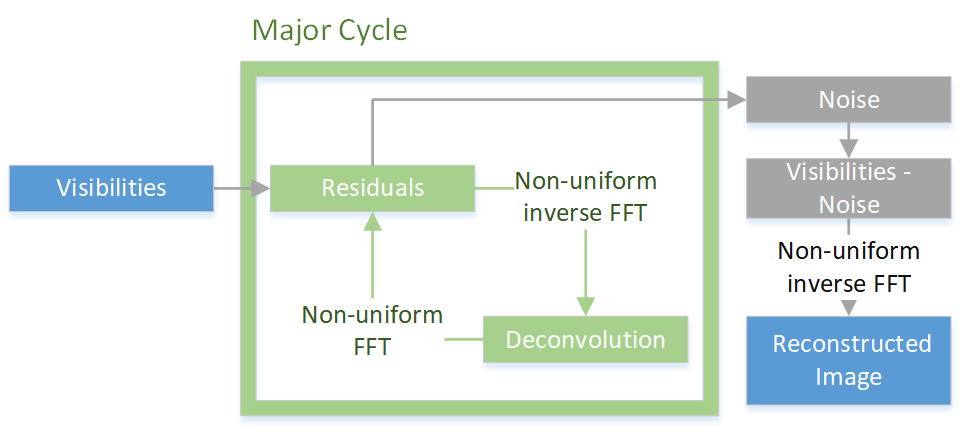
\includegraphics[width=1.0\linewidth]{./chapters/01.intro/Major-Minor.png}
	\caption{The Major Cycle Framework}
	\label{intro:major}
	\vspace{-10pt}
\end{wrapfigure}

The first major cycle uses the non-uniform inverse FFT to approximate the 'dirty' image from the Visibilities. The deconvolution algorithm decides parts which parts belong to the observed image and which are due to instrumental and other noise effects. It returns the noise part of the image, which gets transformed back into residual Visibilities. The next major cycle iteration continues with the residual Visibilities. The residual Visibilities get minimized until they contain only the instrumental effects and noise.

After several major cycles the residual  on a regularly spaced image which has a small error from non-uniform samples, and a small error from incomplete measurements.

Compressed sensing reconstructions essentially use the same architecture, although with minor alterations. In general, they keep a similar scheme of forward/backward non-uniform FFT, but do not use a deconvolution in image pace. Instead, they analyse constraints defined on the image (For example all pixels should be non-negative), and try to find the Visibilities that minimize the constraint violations.

For CLEAN reconstructions, the forward/backward non-uniform FFT are the most expensive operations, while the deconvolution is negligible. The compressed sensing algorithms tend to require more major cycle iterations to converge and the image constraint analysis tends to be more expensive than CLEAN deconvolutions. Current research into compressed sensing reconstructions is focussed on reducing the number of major cycles\cite{dabbech2018cygnus}. 

%Different architecture, but has to somehow handle all the difficulties that arise from imaging meerkat data.


%compressed sensing got rid of the miinor cycle, but essentially kept the major cycle framework
%have to handle own problems in a new architecture







\newpage
\section{Challenges for imaging MeerKAT data} \label{meerkat}
We introduced the basic measurement equation and the imaging problem for Radio Interferometers. MeerKAT introduces a variety of new challenges for image reconstruction. In this work, we limit the scope to the third Fourier term of wide field of view imaging, and discuss the basics of calibration. Both directly affect how the reconstruction algorithm deals with the Fourier Transform and the wider architecture of the reconstruction. In this section, we look at the wide field of view measurement equation, discuss the basics of calibration and how they are solved in the Major Cycle architecture.


\subsection{Wide Field of View Imaging and the third Fourier dimension} \label{meerkat:wof}
In wide field of view imaging, the simplifications we could make from the basic measurement equation \eqref{intro:basic} do not hold. The Visibility space of an interferometer actually has a third $w$-term. This leads us to the wide field of view measurement equation \eqref{meerkat:ftsphere}.

\begin{equation}\label{meerkat:ftsphere}
V(u, v, w) = \int\int \frac{I(x, y)}{\sqrt{1 - x^2 - y ^2}} e^{2 \pi i [ux+vy+ w(\sqrt{1 - x^2 - y ^2} - 1)]} \: dx \: dy
\end{equation}

For a small field of view, the term  $\sqrt{1 - x^2 - y ^2} \approx 1$, which simplifies to our original \eqref{intro:basic}, we can ignore the $w$-term and use the two dimensional Fourier transform. Older interferometers typically created small field of view observations, where the basic measurement equation was accurate enough. But MeerKAT produces wide field of view observations. The $w$-term cannot be ignored anymore and has to be corrected. The figure \ref{meerkat:wcorrection} shows the effect of ignoring the $w$-term for wide-field of view observations. The image gets more distorted away from the center. Emissions at the edges of the image get "torn" apart.

\begin{figure}[h]
	\centering
	\begin{subfigure}[b]{0.45\linewidth}
		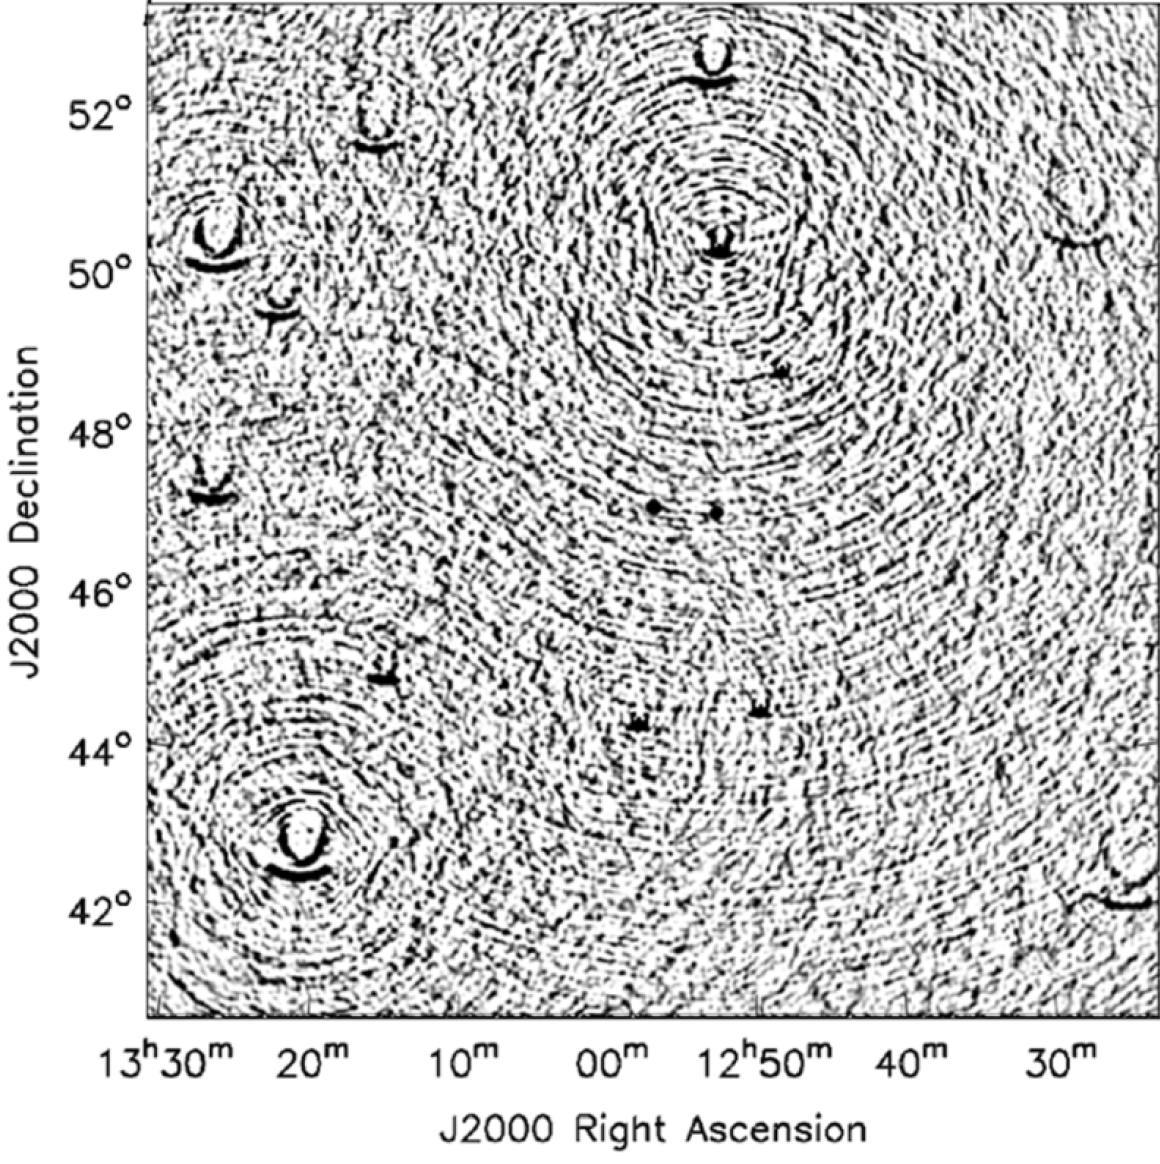
\includegraphics[width=\linewidth]{./chapters/03.challenges/w-no-correction.png}
		\caption{2D Fourier Transform.}
		\label{meerkat:2dfft}
	\end{subfigure}
	\begin{subfigure}[b]{0.45\linewidth}
		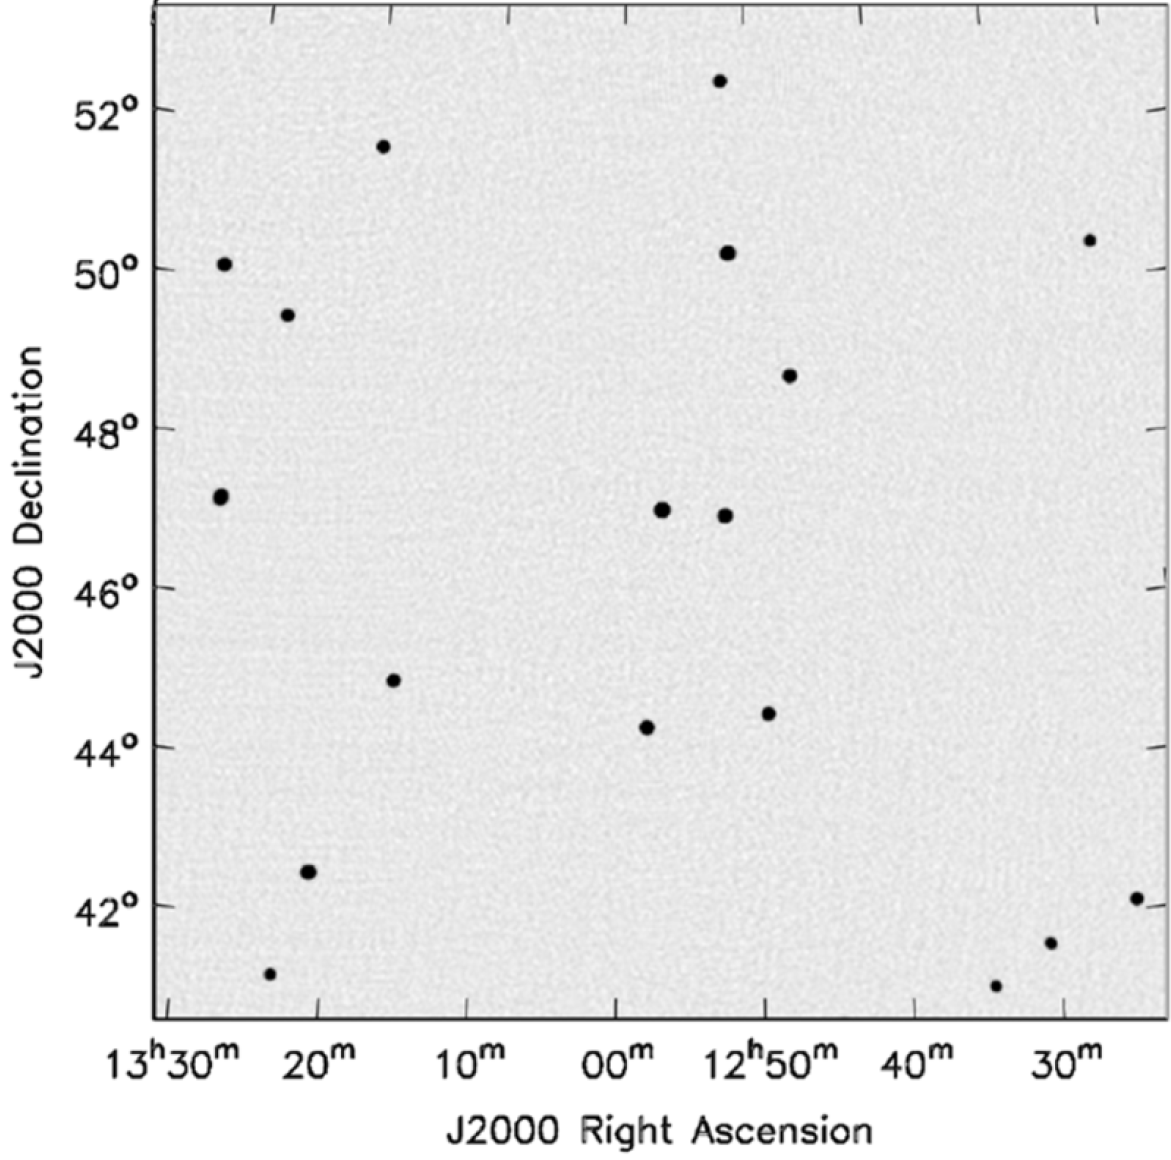
\includegraphics[width=\linewidth]{./chapters/03.challenges/w-correction.png}
		\caption{Fourier Transform with $w$-correction.}
		\label{meerkat:wcorrection}
	\end{subfigure}
	\caption{Celestial sphere distortion on simulated data. Source: \cite{cornwell2008noncoplanar}}
	\label{meerkat:wdistortion}
\end{figure}

Let us look at the wide field of view measurement equation \eqref{meerkat:ftsphere} in detail and explain this phenomenon. We see that the image $I(x,y)$ still two dimensional, even with a three dimensions in Visibility space. The observed image of the interferometer is not on a flat plane, but on a curved surface(hence the $w$-term)\cite{mcewen2011compressed}. More precisely, the instrument looks at the inside wall of the celestial sphere. The two dimensional Fourier transform approximates the curved surface with a flat plane, where the tangent point is typically the image center. The further away we move from the tangent point, the more distortion gets added by the curvature, represented by the term $\sqrt{1 - x^2 - y ^2}$. The curve adds a phase shift the further away we move from the tangent point. If the reconstruction algorithm ignores the $w$-component for a wide field of view, the phase-shift gets severe enough to decorrelate the Visibilities, "tearing" apart the image structures of \eqref{meerkat}.

The effect of the $w$-term is one example of a Direction Dependent Effect (DDE). Wide field of view imaging introduces a number of DDE's, like distortions from the ionosphere and bleed over from different polarization. Correcting for the DDE in the Major Cycle architecture is under research\cite{intema2009ionospheric}, and is therefore out of scope for this project. We only correct for the $w$-term which directly influences the Fourier Transform and the architecture of reconstruction algorithms. 


\subsubsection{State of the art: $w$-stacking algorithm}
The third Fourier breaks the two dimensional relationship between image and Visibilities, which keeps us from using the non-uniform FFT in the Major Cycle architecture. Before the $w$-stacking algorithm was developed, a wide field of view image was faceted into image patches where the $w$-term could be approximated with the small field of view measurement equation. $w$-stacking is the state-of-the-art way of approximating for the $w$-correction in an efficient manner. It calculates a $w$-corrected dirty image from three dimensional Visibilities.

\begin{wrapfigure}{r}{0.7\textwidth}
	\centering
	\vspace{-10pt}
	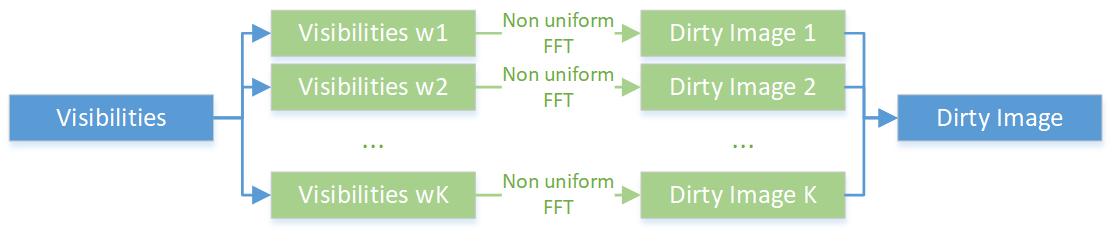
\includegraphics[width=1.0\linewidth]{./chapters/03.challenges/w-stacks.png}
	\caption{The Major Cycle Framework}
	\label{meerkat:w-stacks}
	\vspace{-10pt}
\end{wrapfigure}

The $w$-stacking algorithm, shown in figure \ref{meerkat:w-stacks} replaces the non-uniform FFT. It groups the Visibilities with similar $w$-term into the same layer. Multiple layers are then stacked and transformed independently with the non-uniform FFT. For each stack, the $w$-correction is performed for the center $w$-component. The last step is summing over all stacked images, giving us the final dirty image. From here on a standard CLEAN deconvolution, or a Compressed Sensing algorithm can search for the observed image.

Afterwards, the whole process is reversed. The image gets copied back into the stacks, the $w$-correction gets reversed and the non-uniform FFT calculates the Visibilities per stack.

If we choose uses as many stacks as Visibilities, we end up with an exact $w$-corrections. In practice, many Visibilities have a similar $w$-term. $w$-stacking approximates the correction and allows the Major Cycle to distribute the forward- and backwards non-uniform FFT to a certain extend.

\subsection{Basic Calibration and Self-Calibration}
The Visibilities measured by a Radio interferometer require calibration before an image can be reconstructed. Calibration corrects the amplitude and phase of the measured Visibilities for instrumental differences and direction independent effects. The basic calibration scheme uses a second observation where the true image was known, and solved for the missing calibration parameters $C$, shown in equation \eqref{meerkat:calibration}. $V_2$ are the Visibilities from the calibration observation, and $x_2$ is the known image. The resulting calibration parameters are then used in the observation of interest. 

\begin{equation}\label{meerkat:calibration}
\underset{C}{minimize} \: \left \| CV_2 - F(x_2 \star PSF) \right \|_2^2
\end{equation}

Accurate calibration is necessary for a high-fidelity image reconstruction. For small field of view observations, the number of calibration parameters is relatively small and if the observation spans a short period of time, sufficiently accurate. For observations over a longer time period, the calibration parameters drift significantly, and wide field of view increases the number of necessary parameters. 

The equation \eqref{meerkat:calibration} is essentially the reverse operation of image reconstruction. If we know at least parts of the observed image, we can improve the calibration parameters. This has let to the self-calibration scheme where only an initial calibration is done with a secondary observation, and the imaging algorithm is expected to improve upon the calibration parameters. In self-calibration mode, the imaging algorithm creates a reconstruction from initial calibration. The reconstruction is used to improve the calibration, which in turn gets used for the next reconstruction. The imaging algorithm iteratively solves for both, the observed image $x$ and the calibration parameters $C$.

For wide field of view, observations over a long time period, self-calibration leads to a more accurate reconstruction than otherwise possible. As we will see in the next section, self-calibration has implication on the Fourier Transform of the reconstruction algorithm and therefore on the overall architecture.







\newpage
\section{Alternatives to the non-uniform FFT}\label{killmajor}
The MeerKAT creates wide field of View observations. For accurate image reconstruction, the algorithm also has to optimize the calibration parameters $C$ together with the observed image $x$. This leads us to the following optimization objective \eqref{killmajor:objective} for MeerKAT imaging. $F_{wof}$ represents the wide field of view Fourier Transform with three dimensional Visibilities and two dimensional image. 

\begin{equation}\label{killmajor:objective}
\underset{C, x}{minimize} \: \left \| CV - F_{wof}x \right \|_2^2 + \lambda \left \| P(x) \right \|_1
\end{equation}

State of the art CLEAN algorithms use the Major Cycle architecture for image reconstruction. They use the $w$-stacking algorithm to approximate $F_{wof}$ and cycle between Visibility and image space. Current Compressed Sensing approaches use the $w$-stacking algorithm in a similar manner\cite{girard2015sparse, dabbech2018cygnus, mcewen2011compressed, pratley2018fast}, but need more cycles to converge to an image. This is one reason for the overall higher runtime costs of Compressed Sensing. Various research focuses on improving the reconstructions in the context of the non-uniform FFT and $w$-stacking. Pratley et al\cite{pratley2017robust} optimized the accuracy of the non-uniform FFT for Compressed Sensing reconstructions. Dabbech et al.\cite{dabbech2017wEffect} investigated $w$-term approximations for reducing runtime costs. 

Alternatives to the non-uniform FFT are rarely discussed in Radio Astronomy. We found only Hardy\cite{hardy2013direct} which investigated the direct Fourier Transform for Compressed Sensing reconstructions. In this project, we investigate if we can use an alternative to the non-uniform FFT and reduce the runtime costs of Compressed Sensing. We discuss three alternatives: Optimal projection on a uniform grid, Spherical Harmonics and the direct Fourier Transform.

\subsection{Optimal projection on a uniform grid}
The $w$-stacking algorithm continually cycles between non-uniform Visibility space and uniform image space. Over several cycles a reconstruction algorithm finds the optimal projection on the uniform grid together with the observed image. Here we discuss the potential of searching for the optimal projection first and reconstruct the image in a second step.

\begin{alignat}{1}
\underset{I_{dirty}}{minimize} \:& \left \|  V - \tilde{F}_{wof}I_{dirty} \right \|_2^2\label{killmajor:sep:major}\\
\underset{x}{minimize} \:& \left \| I_{dirty} - x \star PSF \right \|_2^2 + \lambda \left \| P(x) \right \|_1 \label{killmajor:sep:deconv}
\end{alignat}

The first objective \eqref{killmajor:sep:major} solves for the optimal projection on a uniform grid. It uses the $w$-stacking algorithm, represented as $\tilde{F}_{wof}$, which approximates the wide field of view Fourier transform. After we found the optimal projection, we do not need the original Measurements for further processing. The objective \eqref{killmajor:sep:deconv} only needs the dirty image and the Point Spread Function to find the observed image according to some prior $P()$. In this setting, Compressed Sensing reconstructions and CLEAN need the same amount of $w$-stacking cycles.  \eqref{killmajor:sep:major}. 

The main advantage for this architecture is that it reduces the problem to a uniformly-sampled grid, and ignore the original Visibilities in later steps. However, note that \eqref{killmajor:sep:major} and \eqref{killmajor:sep:deconv} do not solve for calibration parameters. $C$ is defined in the non-uniformly sampled space. Unless we find a way to project the calibration problem on a uniform grid too, we cannot ignore the original Visibilities and the main advantage of this setting vanishes. 

In practice, there is a second difficulty with the optimal projection: The $PSF$ of objective \eqref{killmajor:sep:deconv} is difficult to represent accurately on a uniform grid. As mentioned in section \ref{intro:nufft} the $PSF$ varies over the image. For the most accurate result, we would need a $PSF$ for each pixel. The naive way to calculate a $PSF$ for a pixel is to set all amplitudes of our Visibilities to 1, shift the phase to the desired pixel, and calculate the Fourier Transform. The naive way to calculate a $PSF$ for each pixel leads to a quadratic runtime.

CLEAN gets away with a constant $PSF$\footnote{CLEAN implementations in Radio Astronomy typically use a constant $PSF$. This is not necessary, one can also implement CLEAN with a varying $PSF$.}, because of the Major Cycle architecture. In each cycle, it reduces the error it introduced by the constant $PSF$ of the previous cycle, leading to a more accurate reconstruction. When we project on a uniformly sampled grid, we need several $PSF$s for a comparable accuracy to the Major Cycle, and this number dictates whether we can reduce the runtime costs. 

The question, whether projecting on a uniform grid is a viable alternative, depends on how efficiently the $PSF$ can be estimated, and if the calibration parameters can be mapped on a uniform grid. The optimal projection approach is not a viable before we find a way to map the calibration parameters.


\subsection{Spherical Harmonics}
Spherical Harmonics are a different way to represent the measurements of an interferometer. Carozzi\cite{carozzi2015imaging} derived a measurement equation based on the fact that the Visibilities fulfils the Helmholtz equation. In practical terms, Carozzi showed we can replace $F_{wof}$ in our reconstruction problem \eqref{killmajor:objective} the Spherical Harmonics Transform. 

Compared to the Fourier domain, Spherical Harmonics naturally represent wide field of view interferometers and do not have a third dimension. This opens up new designs for Compressed Sensing reconstructions. For example, we can reconstruct the image by in-painting the missing Spherical Harmonics. Because they naturally represent curved surfaces, we can in-paint in a two dimensional space instead of three. Another direction is to image on the sphere directly. MCewen et al.\cite{mcewen2008simulating} showed a way to put two dimensional wavelets on the sphere. A Compressed Sensing reconstruction can use a spherical wavelet as regularization and may simplify the transformation between measurements and reconstruction space.

Sadly, there is little published research in this area for Radio Astronomy image reconstructions. MCewen et al.\cite{mcewen2008simulating} improved the runtime costs of simulations with the spherical Haar wavelet. Later work\cite{mcewen2011compressed} showed a proof-of-concept Compressed Sensing reconstruction projected on the sphere, which improved the image quality. However, it did not use Spherical Harmonics and \cite{mcewen2011compressed} is still based on the Fourier transform. At this point we have not found a proof-of-concept reconstruction algorithm which uses Spherical Harmonics to reduce runtime costs. 

There seems untapped potential for new, cheaper reconstruction algorithms with Spherical Harmonics. But replacing the $F_{wof}$ with the Spherical Harmonics Transform might have wide-ranging consequences. The Fourier relationship, self-calibration, the effect of the ionosphere, everything discussed in section \ref{meerkat} is based on a plane wave arriving at the instrument\cite{thompson1986interferometry, smirnov2011revisiting}. Spherical Harmonics are not. They are derived from a different property of the signal. If we use the Spherical Harmonics Transform, we do not know if we can still solve for the calibration parameters $C$ in \eqref{killmajor:objective}. We may need to re-invent self-calibration, ionosphere distortion and more for Spherical Harmonic reconstructions.


\subsection{Direct Fourier Transform}
The direct Fourier Transform replaces the $w$-stacking algorithm with the full, explicit Fourier Matrix $F_{wof}$. Hardy\cite{hardy2013direct} showed the direct Fourier Transform leads to a simplified reconstruction algorithm which simplifies parallel computing. In this setting, we can calculate the exact wide field of view Fourier Transform from image to Visibility space. For self-calibration, we require a transformation from image to Visibility space which the direct Fourier Transform provides. The downside is of course we need the whole matrix $F_{wof}$ either in memory, or need to re-calculate it on the fly. For MeerKAT reconstructions, where we reconstruct millions of pixels from several billions of Visibilities, the matrix becomes too large for any practical application.

However, the full matrix is not needed. Remember that CLEAN assumes the image is sparse, meaning only a few pixels are non-zero. In practice, even with extended emissions in the image, large regions of pixels are zero. They do not contribute to the reconstruction. We only need to calculate the Transform for non-zero components. With Compressed Sensing, we are not required to reconstruct in the image space. We can use a space where the image can be represented in even fewer non-zero components, reducing the memory requirement and runtime costs of the direct Fourier Transform. In this project, we use starlets as sparse image representation. We investigate if this approach is enough to let the direct Fourier Transform scale to MeerKATs data volume. 


\newpage
\section{Compressed Sensing with direct Fourier Transform\\ and Coordinate Descent}\label{cd}
Instead of using the Major Cycle architecture and approximate the non-uniform FFT approximation, we directly use the Fourier transform matrix $F$. We show the principle of our approach and of Compressed Sensing reconstructions in general at a simplified example. Let us minimize the objective function \eqref{cd:clean}.

\begin{equation}\label{cd:clean}
\underset{x}{minimize} \: \left \| V - Fx \right \|_2^2 + \lambda \left \| x \right \|_1 \\
\end{equation}

The data term $\left \| V - F^{-1}x \right \|_2^2$ forces our image to be similar to the measurements, and the regularization term $\left \| x \right \|_1$ tells us how likely the current reconstruction is to be the true image. The parameter $\lambda$ weights the trade-off between the data and the regularization term. With our term we assume our image contains only a limited number of non-zero pixels.  When the instrument observes stars, they take up a single pixel in the image. In this case, our prior models the true image well, and the theory of compressed sensing states we are virtually guaranteed to find the truly observed image at the minimum of our objective function \eqref{cd:clean}.

We can use a number of different optimization algorithms to optimize \eqref{cd:clean}. Note however in the one dimensional case, where we only have one pixel, the data term of the objective \eqref{cd:clean} forms a parabola and the regularization term a shrink operation\footnote{The shrink operation reduces the magnitude of the pixel by $\lambda$. For example: Pixel $x = -12.4$, $\lambda = 0.6$. The new pixel value after shrinkage follows as $shrink(-12.4, 0.6) = -11.9$}. The optimum for a single pixel can be calculated by solving for the minimum of the parabola first, followed by a shrink operation. With Coordinate Descent we can exploit this property. We fix all pixels except for one and iteratively solve for the current minimum of each pixel. Now when we iterate over all pixels several times, we eventually converge to a solution. The full Coordinate Descent algorithm can be implemented in a few lines of python code:

\begin{lstlisting} 
def coordinate_descent(V_residual, x, lambda, max_iter):
	for k in range(0, max_iter):
		for i in pixels_row:
			for j in pixels_column:
				x_old = x[i, j]
				fourier_column = calculate_fourier_transform(i, j)
				fr = real(fourier_column)
				fi = imag(fourier_column)
				rr = real(V_residual)
				ri = imag(V_residual)
				
				#find apex
				a = sum(fr**2 + 2*fr*fi + fi**2)
				b = sum(fr*rr + fr*ri + fi*rr + fi*ri)
				x_new = b / a + x_old
				
				x_new = shrink(x_new, lambda)
				x[i, j] = x_new
				V_residual = V_residual - fourier_column * (x_new - x_old)
\end{lstlisting}\label{cd:basic}

Coordinate Descent has to iterate over every pixels possibly several times. How quickly Coordinate Descent converges in theory is not well understood. Our optimization function \eqref{cd:clean} falls in the class of quadratic programming with a strictly convex objective. In this case, Coordinate Descent is guaranteed to converge at least linearly\cite{luo1992convergence}. Sadly, real-world objective functions for image reconstruction are often not strictly convex. Usually our image is constrained to have only positive pixels\cite{mcewen2011compressed}, which breaks the strictly convex property of the objective function. In our environment, the convergence guarantees of Coordinate Descent are not well understood in theory.

In practice, Coordinate Descent can be improved with heuristics. Since we assume our image contains only a few stars, a few non-zero pixels, the simple Coordinate Descent algorithm wastes resources checking if the pixel is still zero. A better scheme would be the active set heuristic\cite{friedman2010regularization}: We iterate over every pixel once. Then, for a given number of iterations, we only check the pixels that have changed. This is an improvement, but impossible in the context of MeerKAT. We have too many pixels and Visibilities, iterating over every pixel once is too expensive. 

However, it turns out we do not need to if we imitate CLEAN: For CLEAN, the non-uniform FFT approximates the 'dirty' image, which is corrupted by the effects of incomplete measurements. CLEAN then subtracts a fraction of the PSF at the largest pixel value. In other words, the largest pixel value in the dirty image is the most likely non-zero pixel. We can use the dirty image approximation for a 'probability distribution' of non-zero pixels. It does not need to be accurate, since the actual reconstruction is done with the direct Fourier Transform.

This is, in principle, how the proof-of-concept algorithm works. Instead of reconstructing an image, it reconstructs in the starlet space. It uses the starlet transform of the dirty image to find likely non-zero components. Coordinate Descent is used to optimize single starlets. A proof-of-concept version of this algorithm was developed in python.

Although the algorithm produces super-resolved images in section \ref{results}, it is currently not known if it actually converges to the true optimum. Finding all relevant non-zero starlets is left to a greedy heuristic. There may be conditions under which it never includes relevant components. Further convergence analysis was outside the scope of the project. Also note that for this implementation, every time likely non-zero components are searched, it simply uses the non-uniform FFT for the dirty image approximation. This was done for simplicity's sake and can be improved.


\subsection{The Starlet Transform} \label{cd:starlets}

\begin{figure}[h]
	\centering
	\begin{subfigure}[b]{0.4\linewidth}
		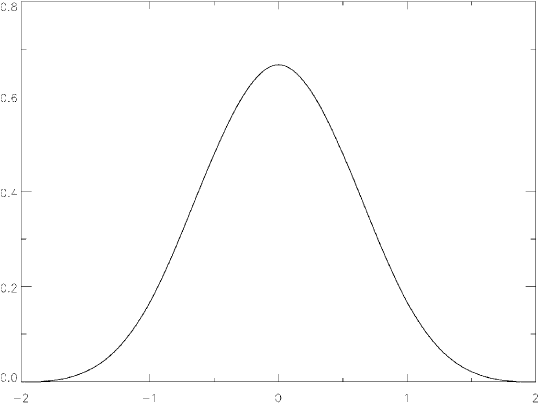
\includegraphics[width=\linewidth]{./chapters/05.algorithms/starlets/scaling.png}
		\caption{Spline scaling function}
		\label{cd:starlets:scaling}
	\end{subfigure}
	\begin{subfigure}[b]{0.4\linewidth}
		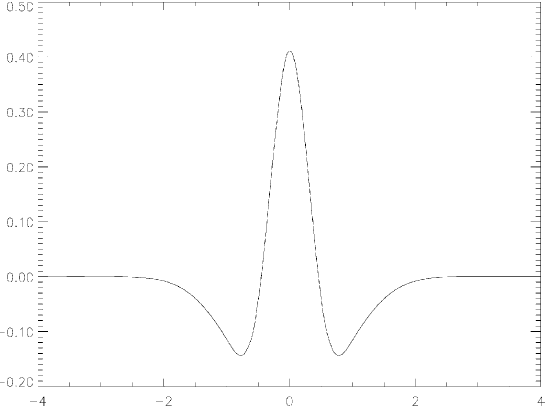
\includegraphics[width=\linewidth]{./chapters/05.algorithms/starlets/wavelet.png}
		\caption{Wavelet function}
		\label{cd:starlets:wavelet}
	\end{subfigure}
	\caption{Scaling and wavelet function of the starlet wavelet. Source: \cite{starck2015starlet}}
	\label{cd:starlets:figure}
\end{figure}

The starlet transform is an Isotropic Undecimated Wavelet Transform (IUWT) with the starlet wavelet shown in figure \ref{cd:starlets:figure}. As such, it defines two operations: The transformation from starlet into image space which is called synthesis, and the inverse which is called decomposition. The starlet space represents an image in multiple layers at different scales, where lower layers contain smaller objects and upper layers the extended emissions. The lowest starlet layer represents the stars, while the upper layer represents the largest hydrogen clouds in the image.

\begin{equation}\label{cd:starlet:w0}
\begin{aligned}
	c_0 &= \bm{x} \star B_0 \\
	\bm{w_0} &= \bm{x} - c_0
\end{aligned}
\end{equation}

Let us look at the lowest starlet layer first, and how it is calculated from the image.
B, and x.
x - c0 removes the larger structures from the image, leaving us with the smallest in $w_0$. Does are not the starlet components, $\alpha_0$. However, we can estimate them with a shrink operation.
we can then convolve $\alpha$ with the starlet function to get back to $w_0$.  In our implementation


In this case, we use it for estimating likely non-zero $\alpha$. Figure \ref{cd:heuristic:figure} shows an example for the lowest starlet layer.

\begin{figure}[h]
	\centering
	\begin{subfigure}[b]{0.4\linewidth}
		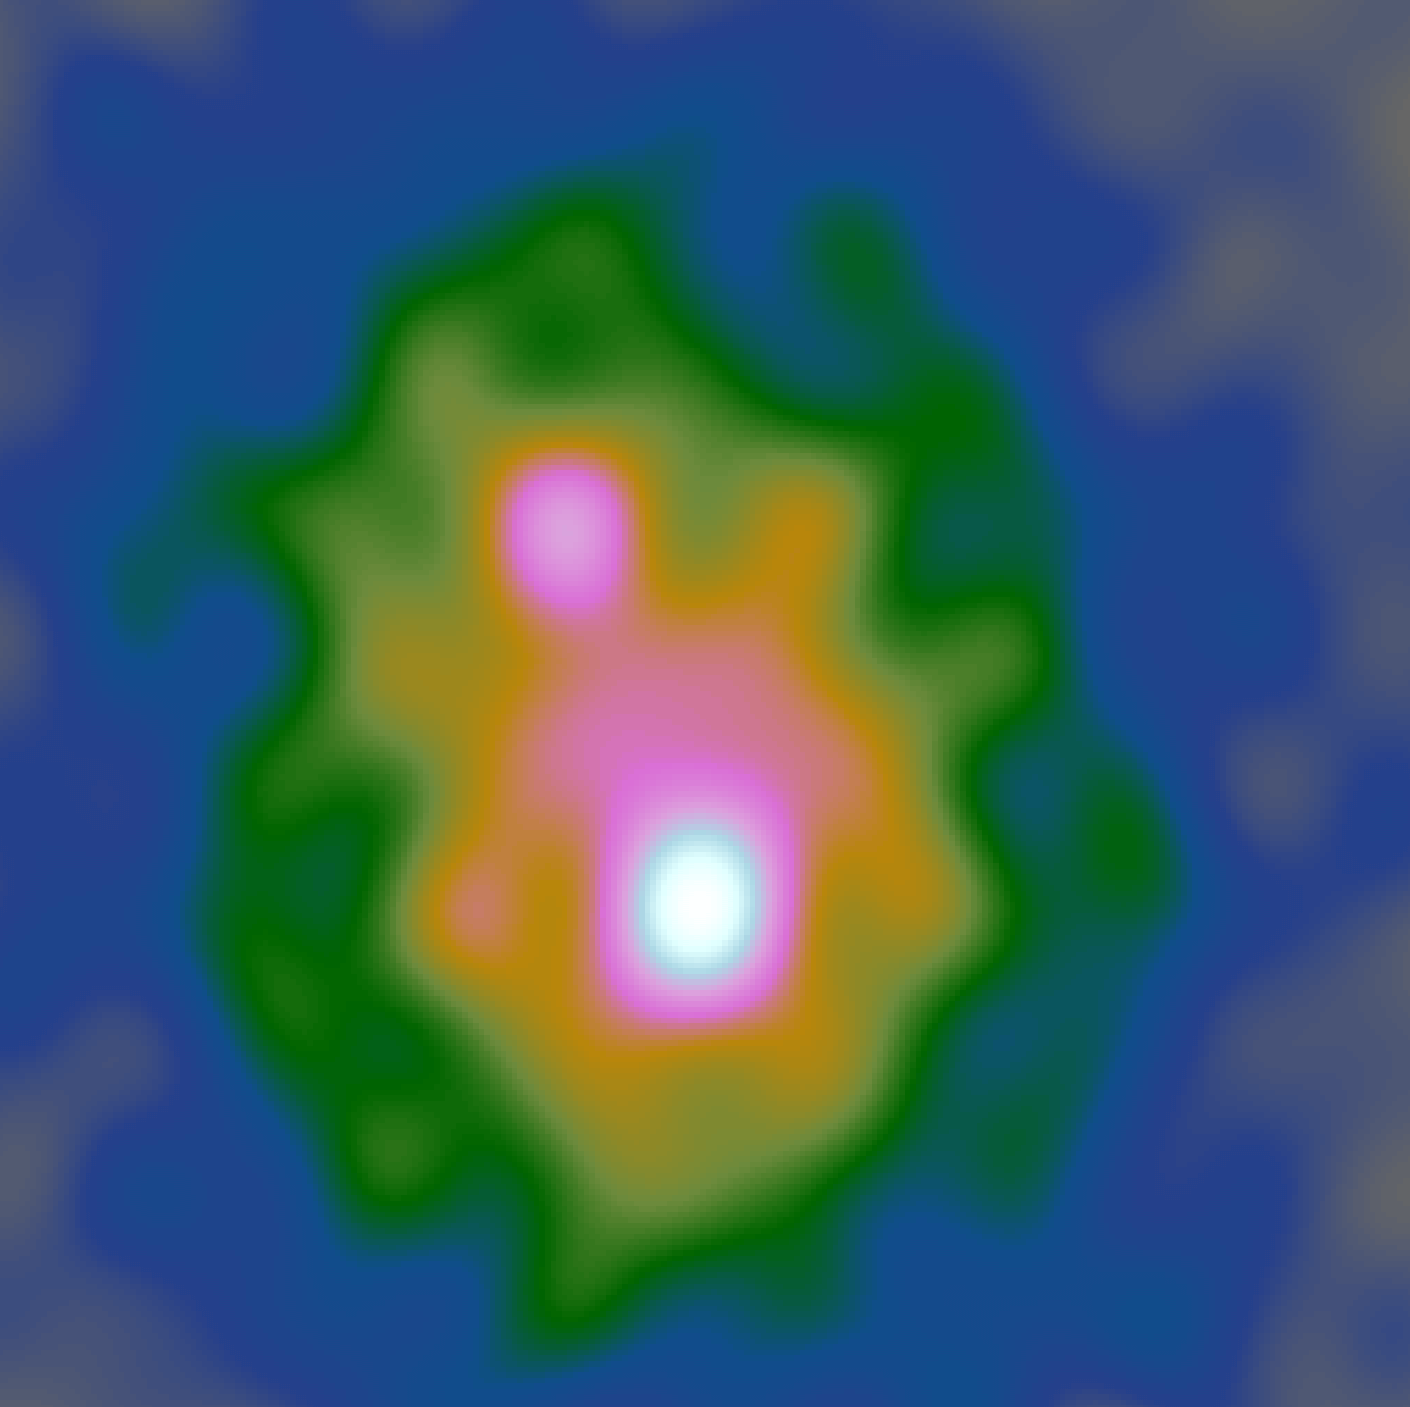
\includegraphics[width=\linewidth]{./chapters/05.algorithms/starlets/dirty2.png}
		\caption{Dirty Image with two point sources.}
		\label{cd:heuristic:dirty}
	\end{subfigure}
	\begin{subfigure}[b]{0.4\linewidth}
		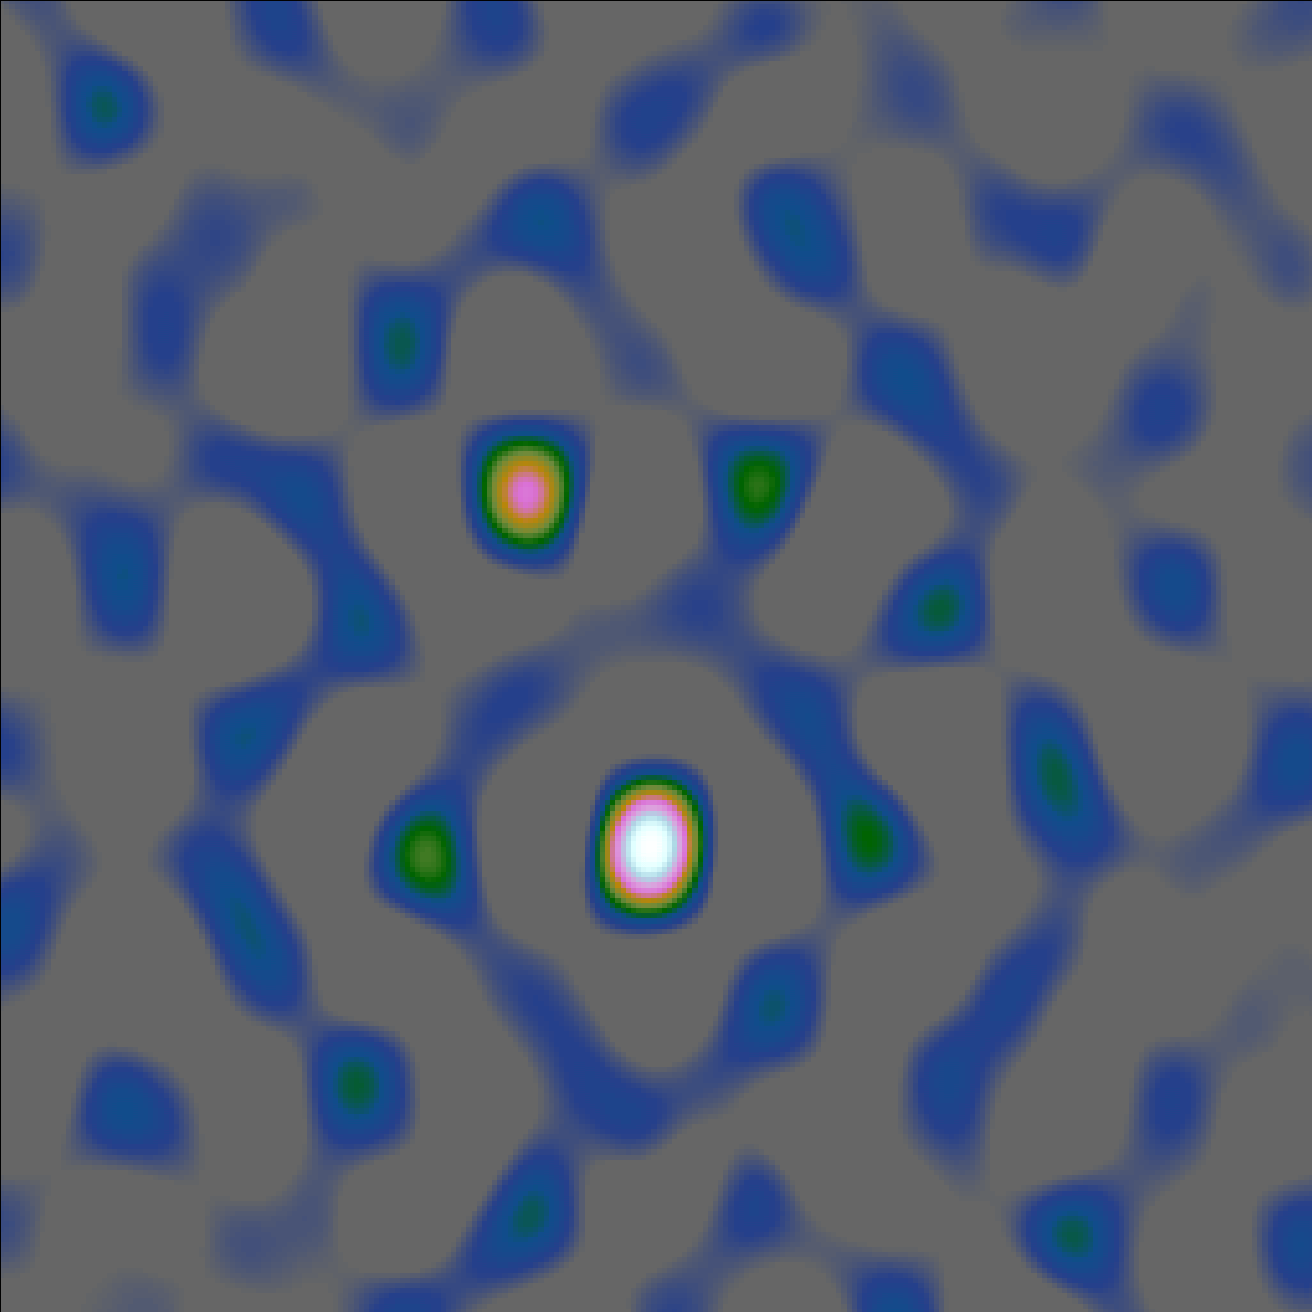
\includegraphics[width=\linewidth]{./chapters/05.algorithms/starlets/starlet0_2.png}
		\caption{Layer $w_0$ of the starlet decomposition.}
		\label{cd:heuristic:starlet}
	\end{subfigure}
	\caption{Dirty map and $w_0$ starlet layer. The right image shows the probability distribution for point sources in the dirty image.}
	\label{cd:heuristic:figure}
\end{figure}


The full decomposition is then just repeated for each intermediate layer $w_i$. \eqref{cd:starlet:decomposition}
!!!!!A trous algorithm, size of the differtent $S_i$
The last, heavily blurred $c_J$ contains the structures which were too big to represent with the largest starlets, and is the last layer of the decomposition.

\begin{equation}\label{cd:starlet:decomposition}
	\begin{split}
		c_0 &= \bm{x} \star B_0 \\
		\bm{w_0} &= \bm{x} - c_0
	\end{split}
	\qquad
	\begin{split}
		c_1 &= c_0 \star B_1 \\
		\bm{w_1} &= c_0 - c_1
	\end{split}
	\qquad \ldots \qquad
	\begin{split}
		c_{J-1} &= c_{J-2} \star B_{J-1} \\
		\bm{w_{J-1}} &= c_{J-2} - c_{J-1}
	\end{split}
	\qquad
	\begin{split}
		\bm{c_J} &= c_{J-1} \star B_J
	\end{split}
\end{equation}

The synthesis transform however is easy.

\begin{equation} \label{cd:starlet:backwards}
\bm{x} = \bm{w_0} + \bm{w_1} + \ldots + \bm{w_{J-1}} + \bm{c_J}
\end{equation}

The starlet decomposition is over-complete.

The difference between $\alpha$ and $w_i$ is not always important. For the SASIR algorithm,  for FISTA, which is how \cite{girard2015sparse} used the starlet transform for regularization, shrinkage on $w_i$ without convolution.

For FISTA, this is irrelevant, but for Coordinate descent it is important. note on the shrinkage


the original starlet people \cite{starck2015starlet} does not differentiate between $\alpha$ and $w_i$, and neither did \cite{girard2015sparse}. For the Coordinate Descent implementation it is relevant for handling the positivity constraint.

\subsubsection{Handling the positivity constraint}
As mentioned in section \ref{cd}, image reconstruction algorithms for radio astronomy typically constrain the image to be non-negative\cite{mcewen2011compressed}.


\subsection{Coordinate Descent Implementation}
We have the starlet regularization, let us put it into an algorithm. Start with the 

\begin{equation}\label{cd:starlet}
\underset{\alpha}{minimize} \: \left \| V - FD\alpha \right \|_2^2 + \lambda \left \| \alpha \right \|_1 \\
\end{equation}

Proof of concept implementation. There are many ways to improve the efficiency and the convergence speed. It is here to show  the general if it is possible of the approach and if we can truly only calculate a subset of $F^{-1}$ columns.

The objective function \eqref{cd:starlet} minimizes the starlet components $\alpha$. This objective leads again to a parabola in the one dimensional case, and we can analytically find the optimum for a single component when all others are fixed. 



There are still a few problems to solve, like how to handle the matrix product $F^{-1}D$, 
With the active set heuristic, we iterate over a limited number of starlet components at a time. 

The question remains, how the matrix product $F^{-1}D$ can be calculated efficiently. Since starlet transform is just made up of a couple of convolutions, we do not have to calculate the product $F^{-1}D$ explicitly. Convolutions in image space are multiplications in Fourier space. 
So for any starlet layer $w_i$ or $c_J$, we can pre-calculate a transform vector. 
$w_2 = F^{-1}V * (\hat{S_0}\hat{S_1} - \hat{S_0}\hat{S_1}\hat{S_2})$

How many layers are needed. starlets rise in pixels with $2^J$. Meaning if we want starlets over the whole image, the number of starlets rise logarithmically to the image dimensions.

How to iterate over the image in detail.



\subsection{Iteration scheme}
Many ways to iterate over the image. A simple scheme was used here. 

Active set heuristic, find the starlets which are 

\begin{lstlisting} 
def coordinate_descent(V_residual, x, lambda, max_iter):
	for k in range(0, max_iter):
		for i in pixels_row:
			for j in pixels_column:
				x_old = x[i, j]
				fourier_column = calculate_fourier_transform(i, j)
				fr = real(fourier_column)
				fi = imag(fourier_column)
				rr = real(V_residual)
				ri = imag(V_residual)
				
				#find apex
				a = sum(fr**2 + 2*fr*fi + fi**2)
				b = sum(fr*rr + fr*ri + fi*rr + fi*ri)
				x_new = b / a + x_old
				
				x_new = shrink(x_new, lambda)
				x[i, j] = x_new
				V_residual = V_residual - fourier_column * (x_new - x_old)
\end{lstlisting}\label{cd:implementation}

coordinate descent with active set heuristic


sub-zero pixels

\subsubsection{Non-uniform FFT approximations}
Non uniform FFT to calculate the convolution KERNELS!!


Stupid approach with line search. Could be done more efficiently by using the histogram of the starlet level.


\newpage
%\section{Benchmark}

\subsection{Data}
\subsubsection{Simulations}

\subsubsection{Real world MeerKAT data}

\subsection{Evaluation Measures}


%\newpage
\section{Coordinate Descent reconstructions on Simulated Data}\label{results}
Here we test the Coordinate Descent algorithm on two simulated datasets and show we indeed only need a subset of the Fourier Transform Matrix' columns $F^{-1}$. The datasets contain idealized MeerKAT observations. Compared to the real world, the two simulated datasets contain few Visibilities and not representative of the real data volume. Also, more realistic simulations which contain pointing-, calibration-, and thermal noise are out of scope for this project. The simulations are used to isolate the two fundamental issues in radio interferometer image reconstruction: Non-uniform sampling and incomplete measurements.

We compare the reconstruction quality to CASA's CLEAN implementation. Coordinate Descent was able to produce a super-resolved version of the simulated measurements, reconstructing point sources above the accuracy limit of MeerKAT.

\subsection{Super-resolution of two point sources}
The first simulated observation contains two non-zero pixels, i.e. point sources, with intensity of 2.5 and 1.4 Jansky/Beam, with a resolution of 0.5 arc-seconds per pixel. The resolution of the image is therefore higher than MeerKAT. An ideal compressed sensing reconstruction would create an image where all pixels are zero except for the two point sources. Figure \ref{results:points} shows the reconstructed images of CLEAN and Coordinate Descent.

CLEAN reconstructs the image \ref{results:points:tclean} at the accuracy limit of the instrument. It essentially reconstructs a blurred version of the observed image, where the blurring represents the accuracy of the instrument. With compressed sensing, we aim to reconstruct a de-blurred image. The image \ref{results:points:cd} shows the Coordinate Descent reconstruction, which creates two much narrower peaks than CLEAN. This is an example of super resolution. Coordinate Descent located structures smaller than the accuracy of MeerKAT would allow.

\begin{figure}[h]
	\centering
	\begin{subfigure}[b]{0.4\linewidth}
		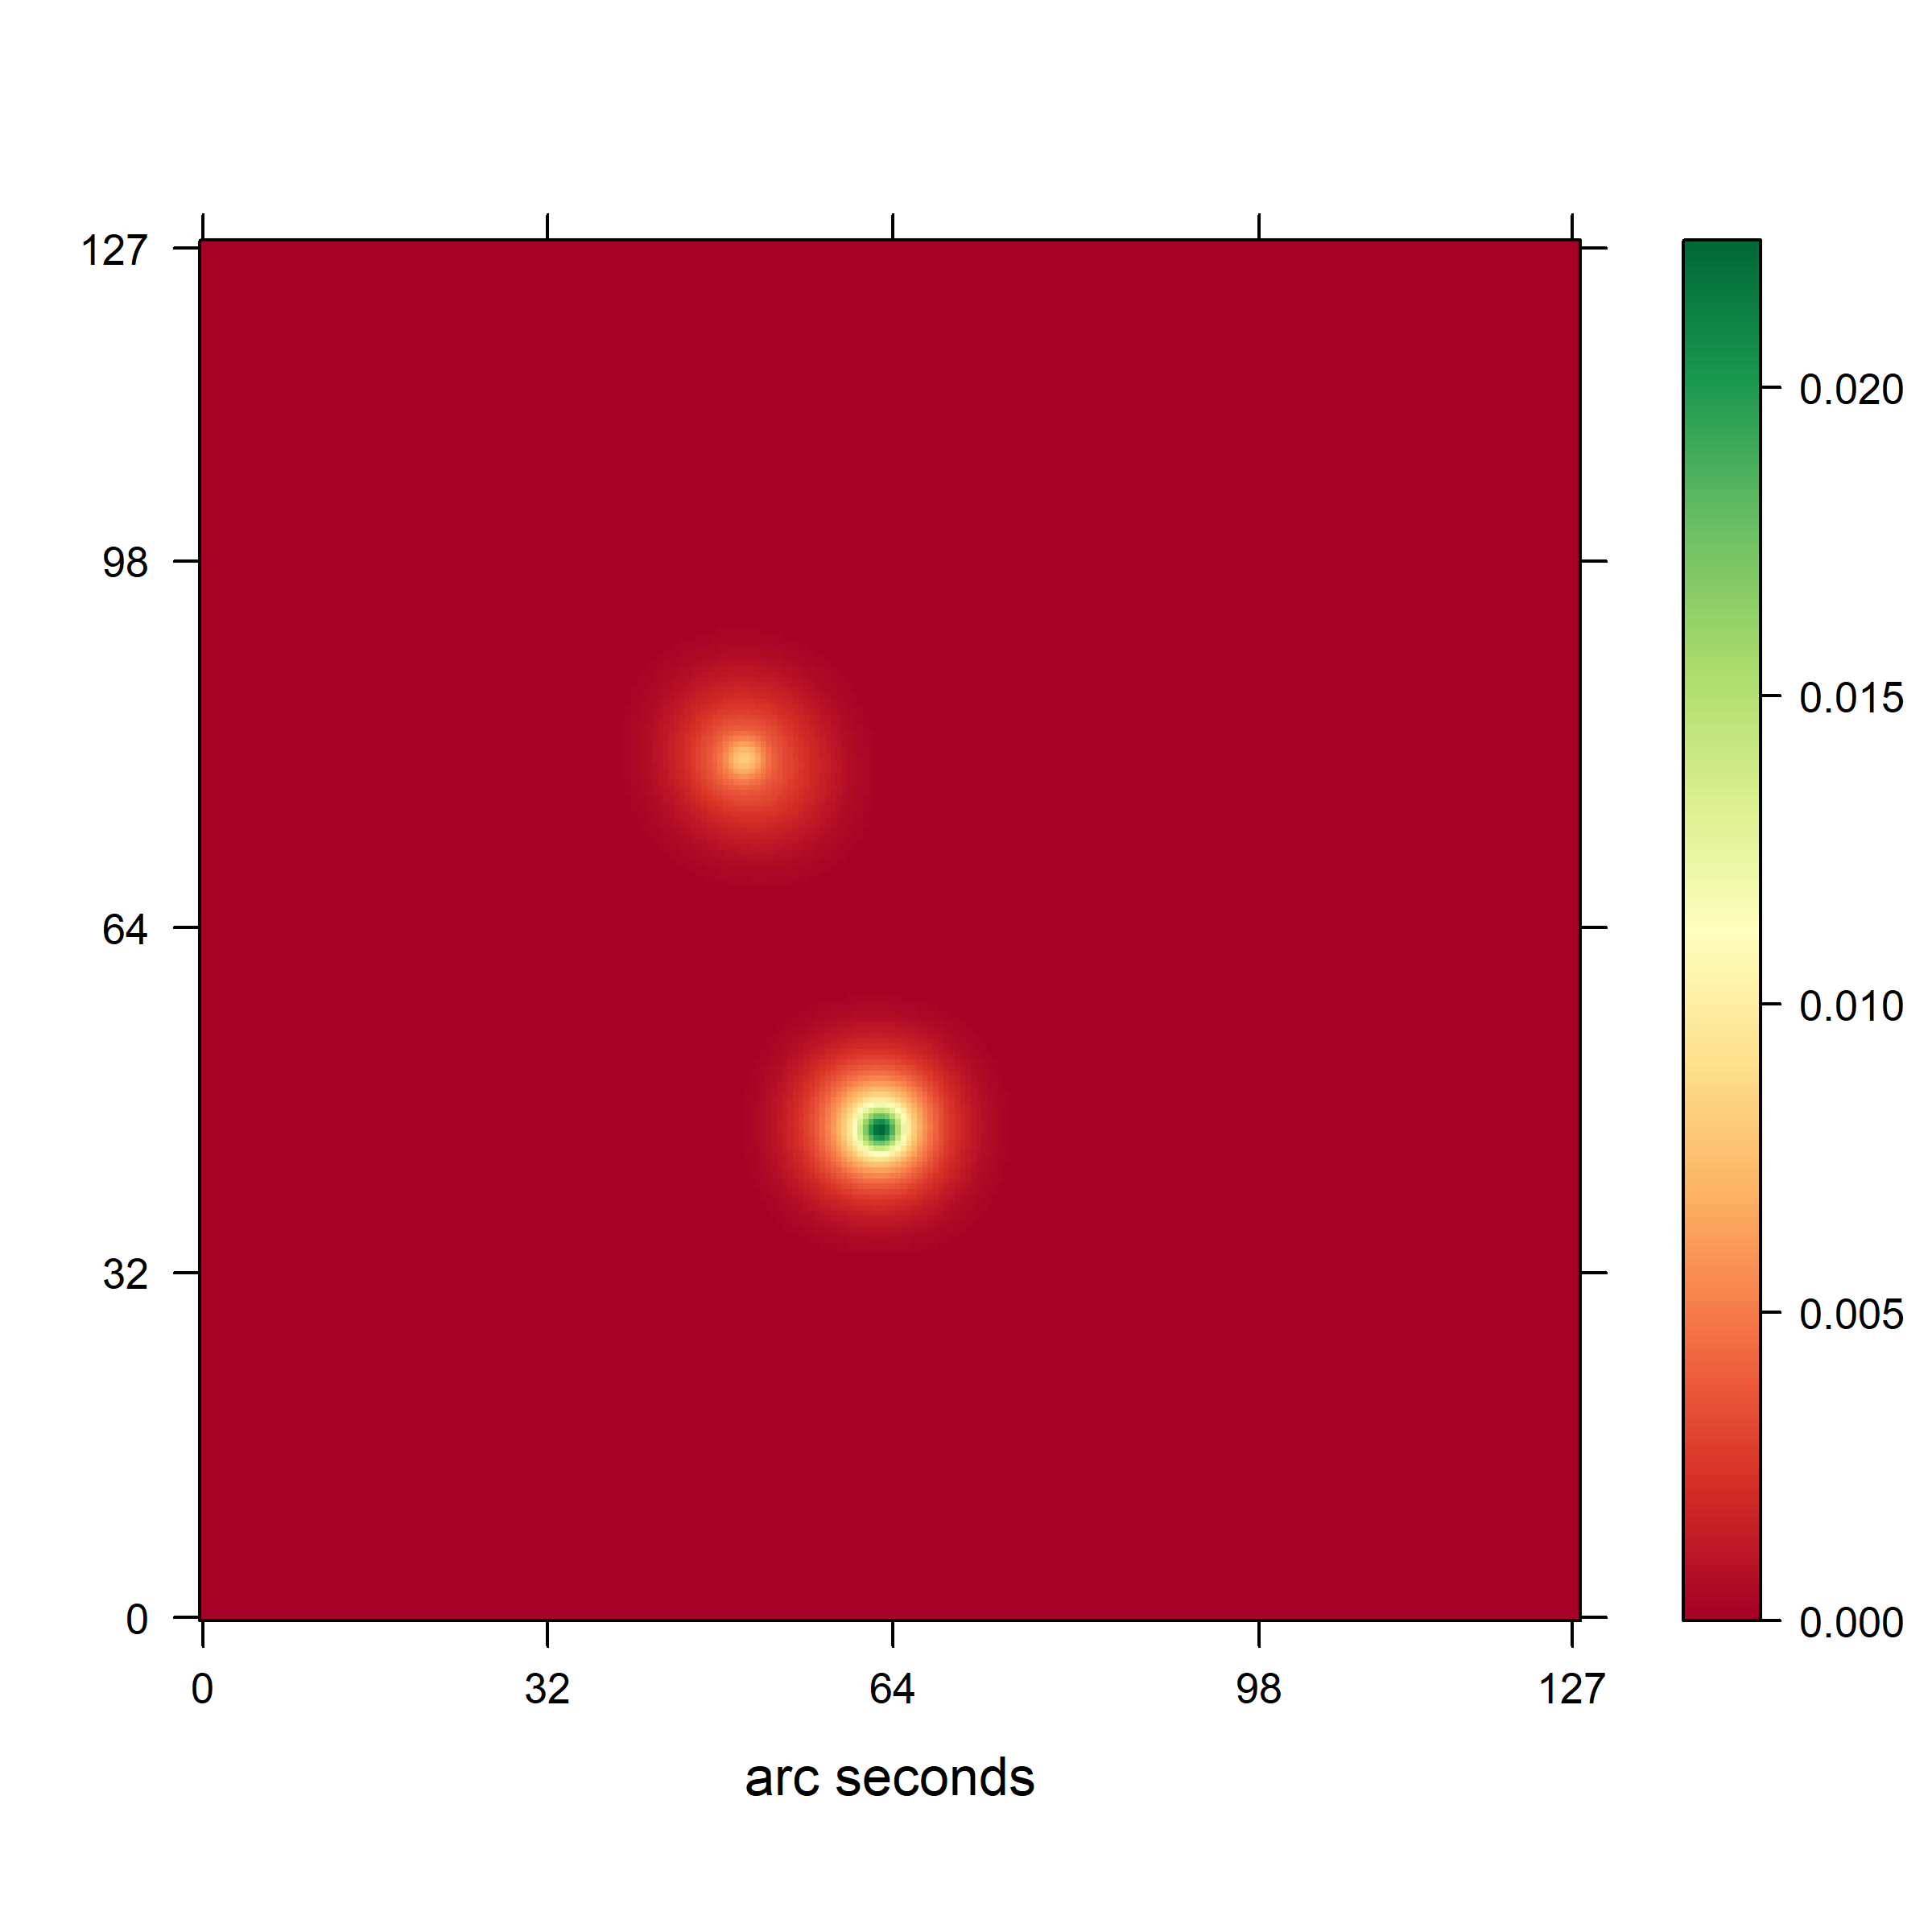
\includegraphics[width=\linewidth, trim={0.2in, 0.2in, 0, 0.2in}, clip]{./chapters/20.results/points/tclean_points.png}
		\caption{CLEAN reconstruction \\with CASA standard parameters.}
		\label{results:points:tclean}
	\end{subfigure}
	\begin{subfigure}[b]{0.4\linewidth}
		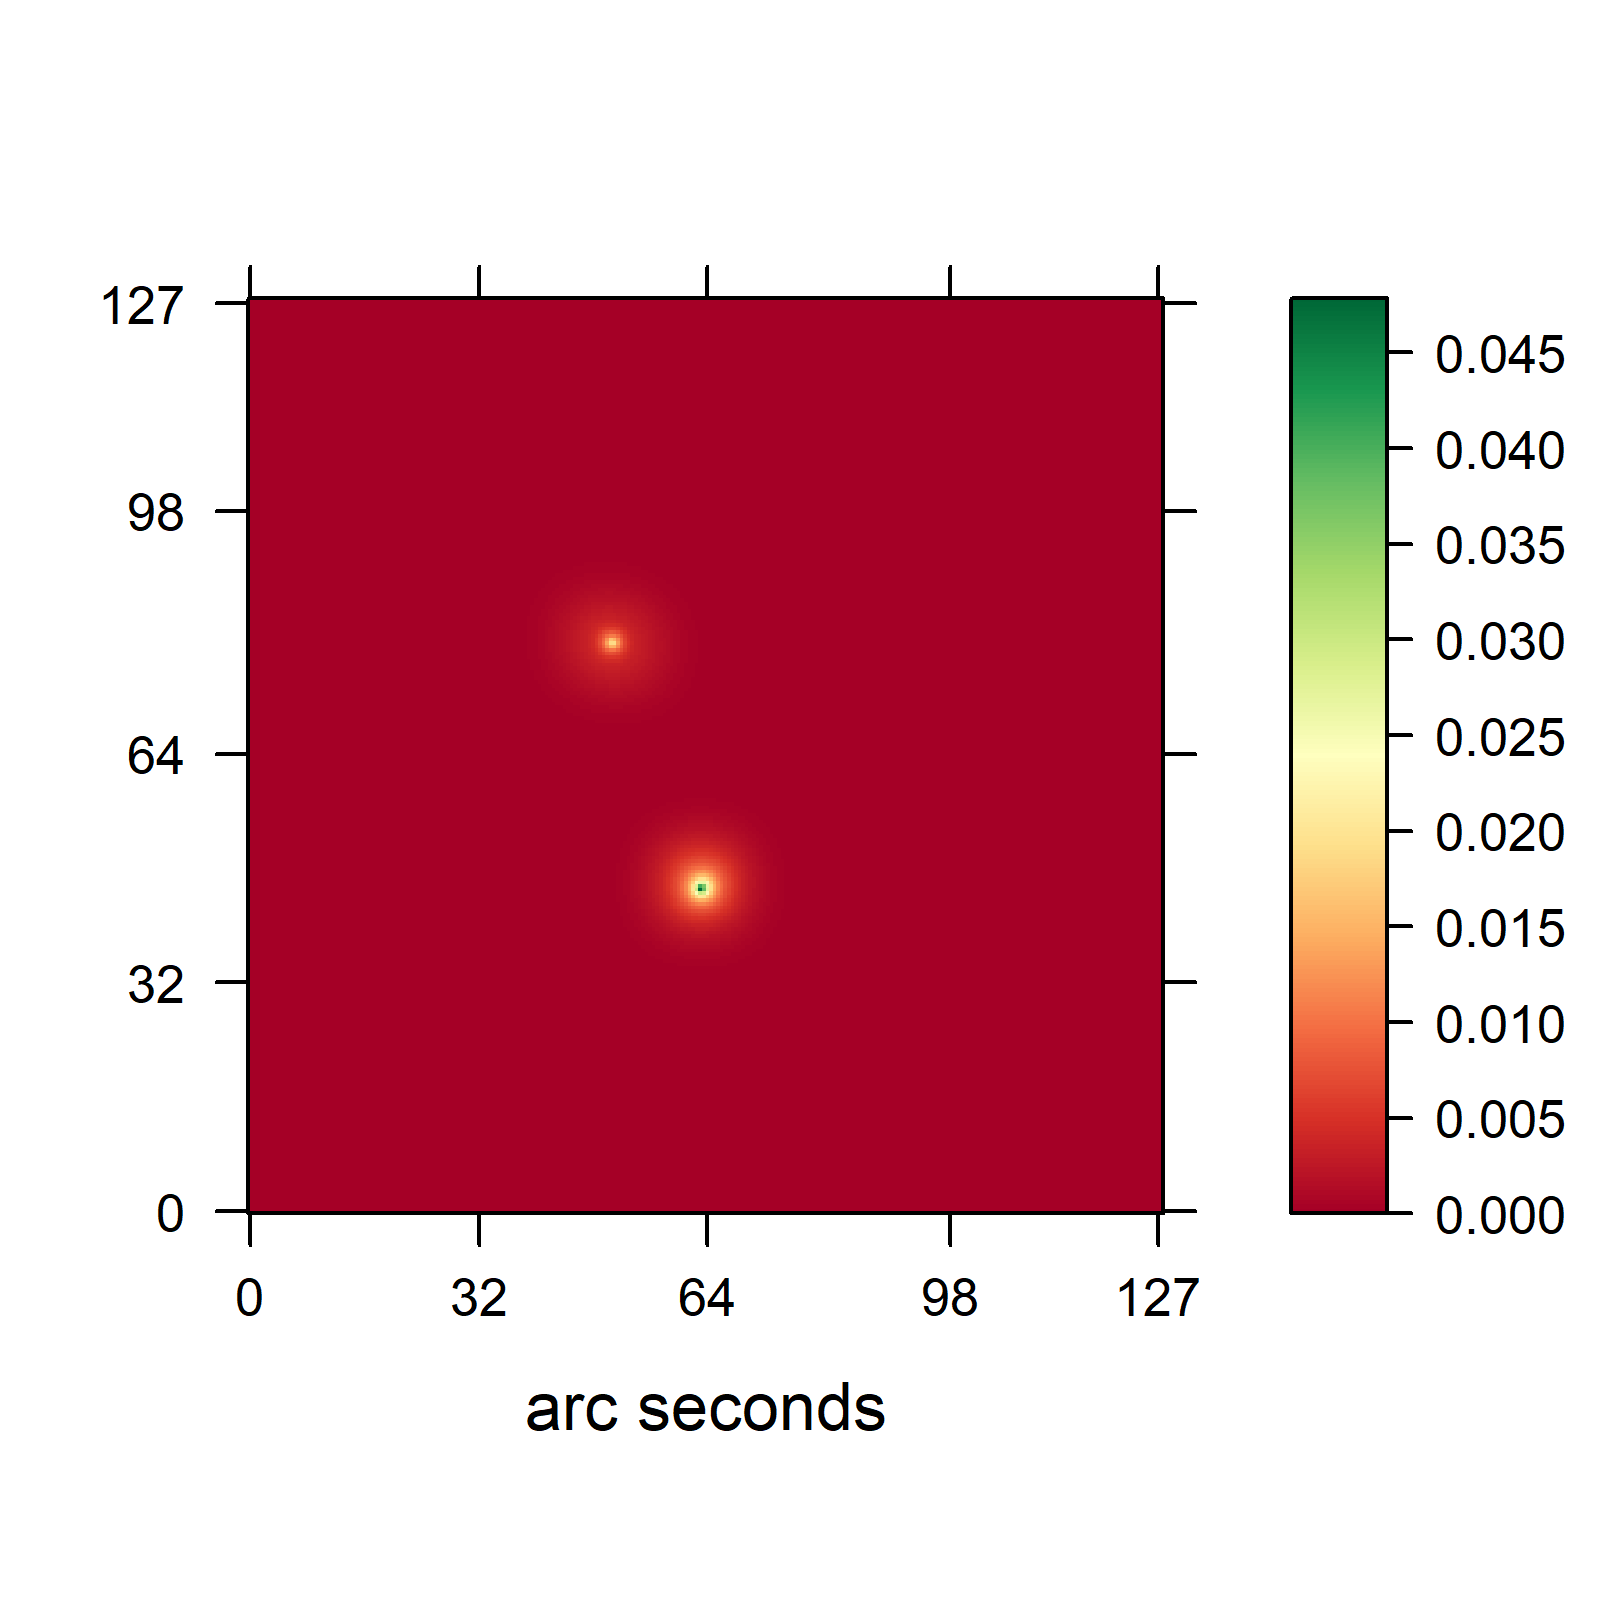
\includegraphics[width=\linewidth, trim={0.2in, 0.2in, 0, 0.2in}, clip]{./chapters/20.results/points/cd_points.png}
		\caption{Coordinate Descent reconstruction\\ with $\lambda = 0.01, J=4$.}
		\label{results:points:cd}
	\end{subfigure}
	
	\caption{Image reconstruction of two point sources.}
	\label{results:points}
\end{figure}

The total Flux of the image, the sum of all emissions, is 3.9 Jansky/Beam in this simulation. CLEAN reconstructs the right peak intensities, both ending up at 2.5 and 1.4 respectively. Since CLEAN reconstructs a blurred version, the total Flux of the image is off by magnitudes. Figure \ref{results:points:contour} compares the intensity profile of CLEAN, Coordinate Descent and the Ground Truth. Note the logarithmic y scale. For a correct total flux, the integrals should be equal. 

\begin{figure}[h]
	\centering
	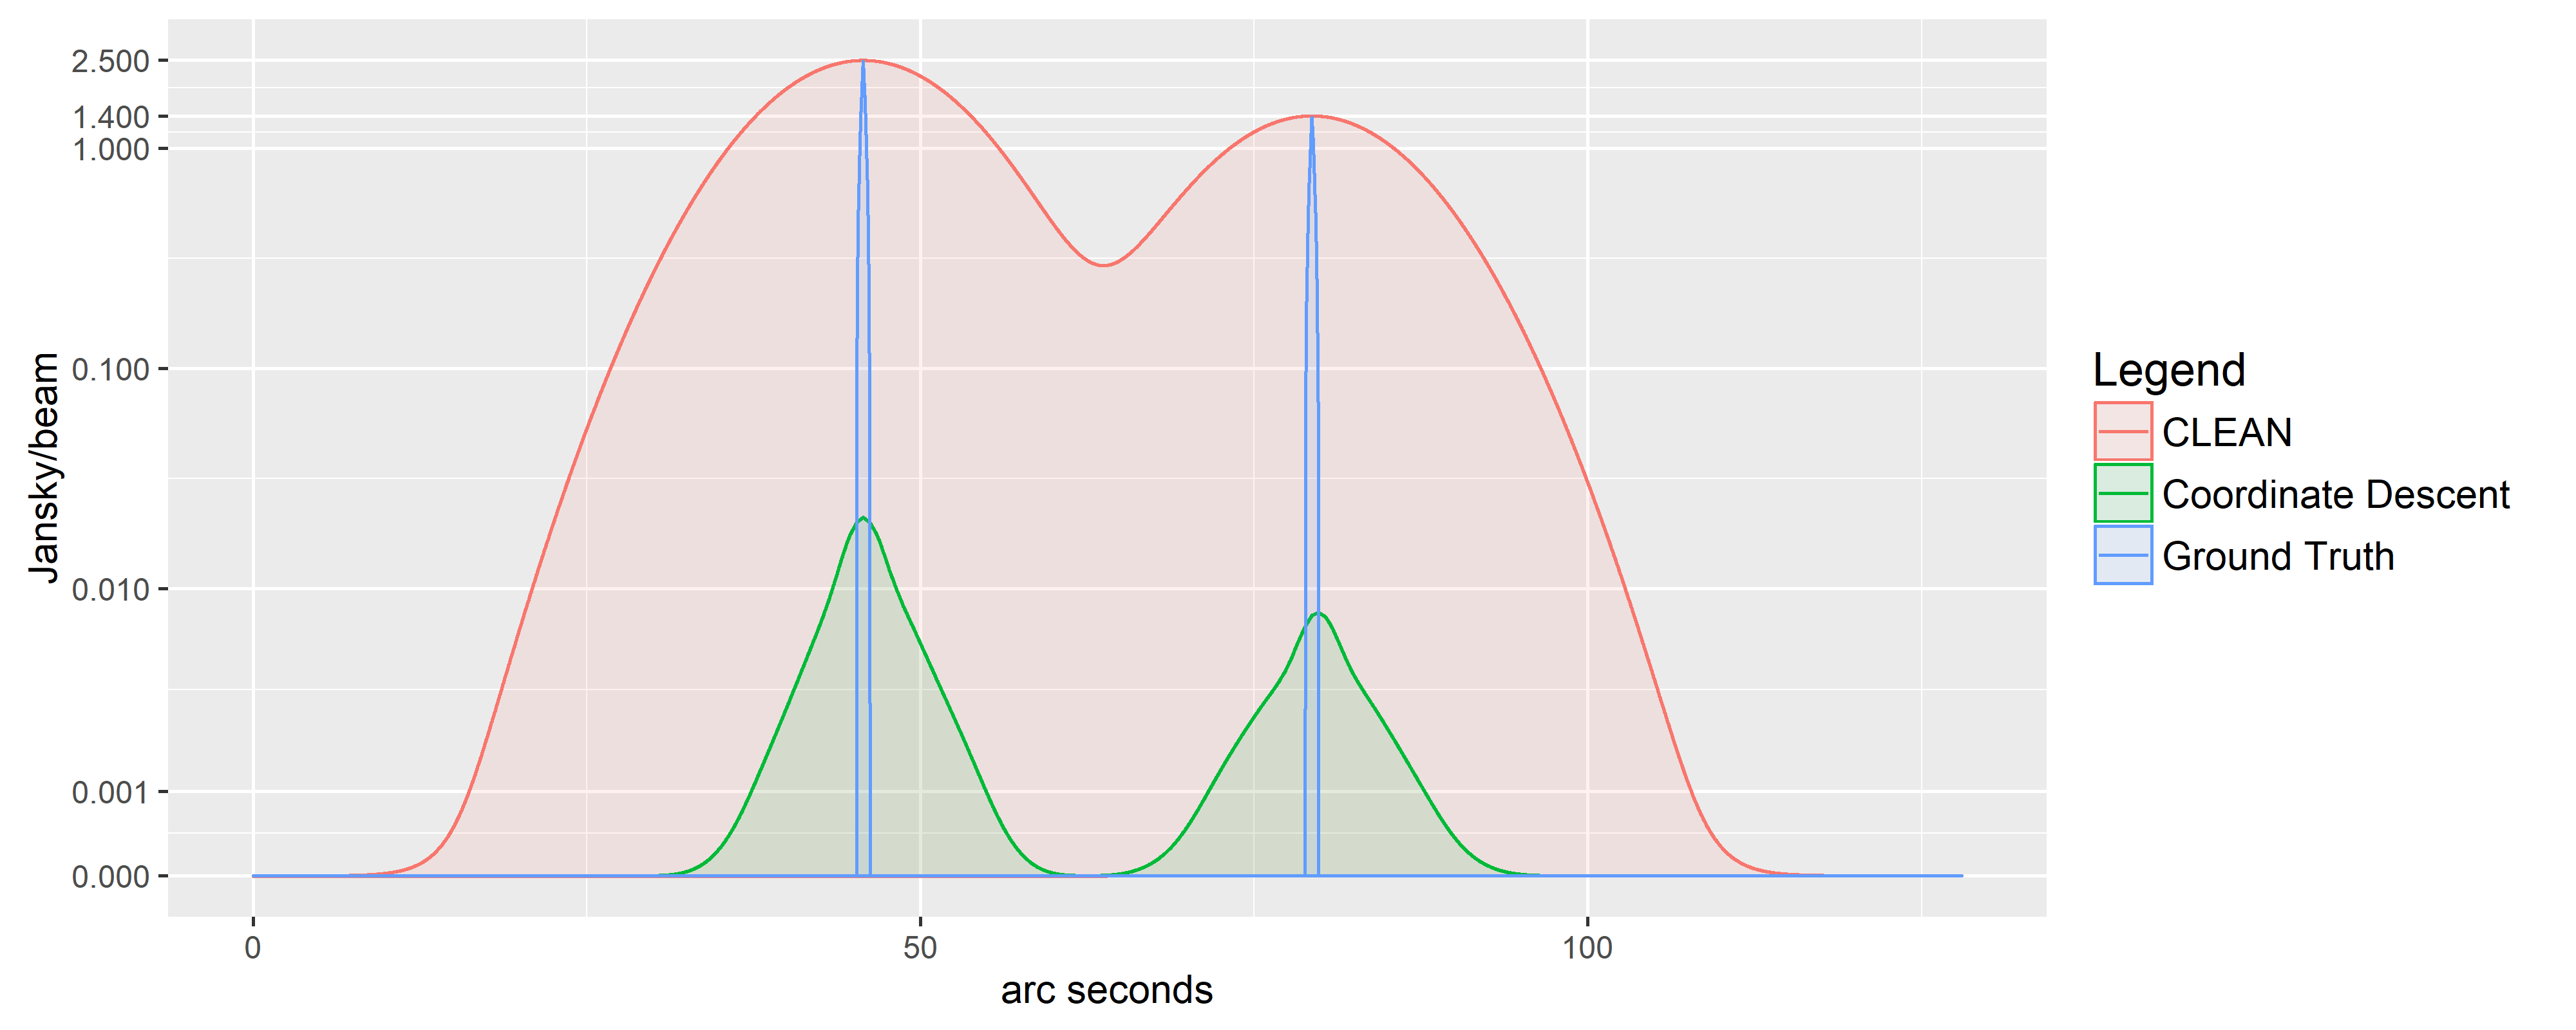
\includegraphics[width=0.8\linewidth]{./chapters/20.results/points/contour_points.png}
	\caption{Intensity profile of the two point sources.}
	\label{results:points:contour}
\end{figure}

In the contour plot, the Coordinate Descents narrow contours become apparent.

The flux is sadly not correct, it seeems to be too large by a factor of two

The larger source was well reconstructed. The second, smaller emissions however has a few issues.

note that the smaller emission is shifted by a pixel and the contour is wider than it's larger cousin. 

The last issue it has that the flux is still not correct. It is close and seems to bigger than a factor of two.



Look at the flux in a more complex environment


\subsection{Flux reconstruction of mixed sources}

Dataset of three gaussian extended emissions and sixteen point sources at varying intensities.

Parameters of Coordinate Descent

super resolution of CD. However, it did not find all point sources
Lets look closer at the flux reconstruction of extended emissions

\begin{figure}[h]
	\centering
	\begin{subfigure}[b]{0.4\linewidth}
		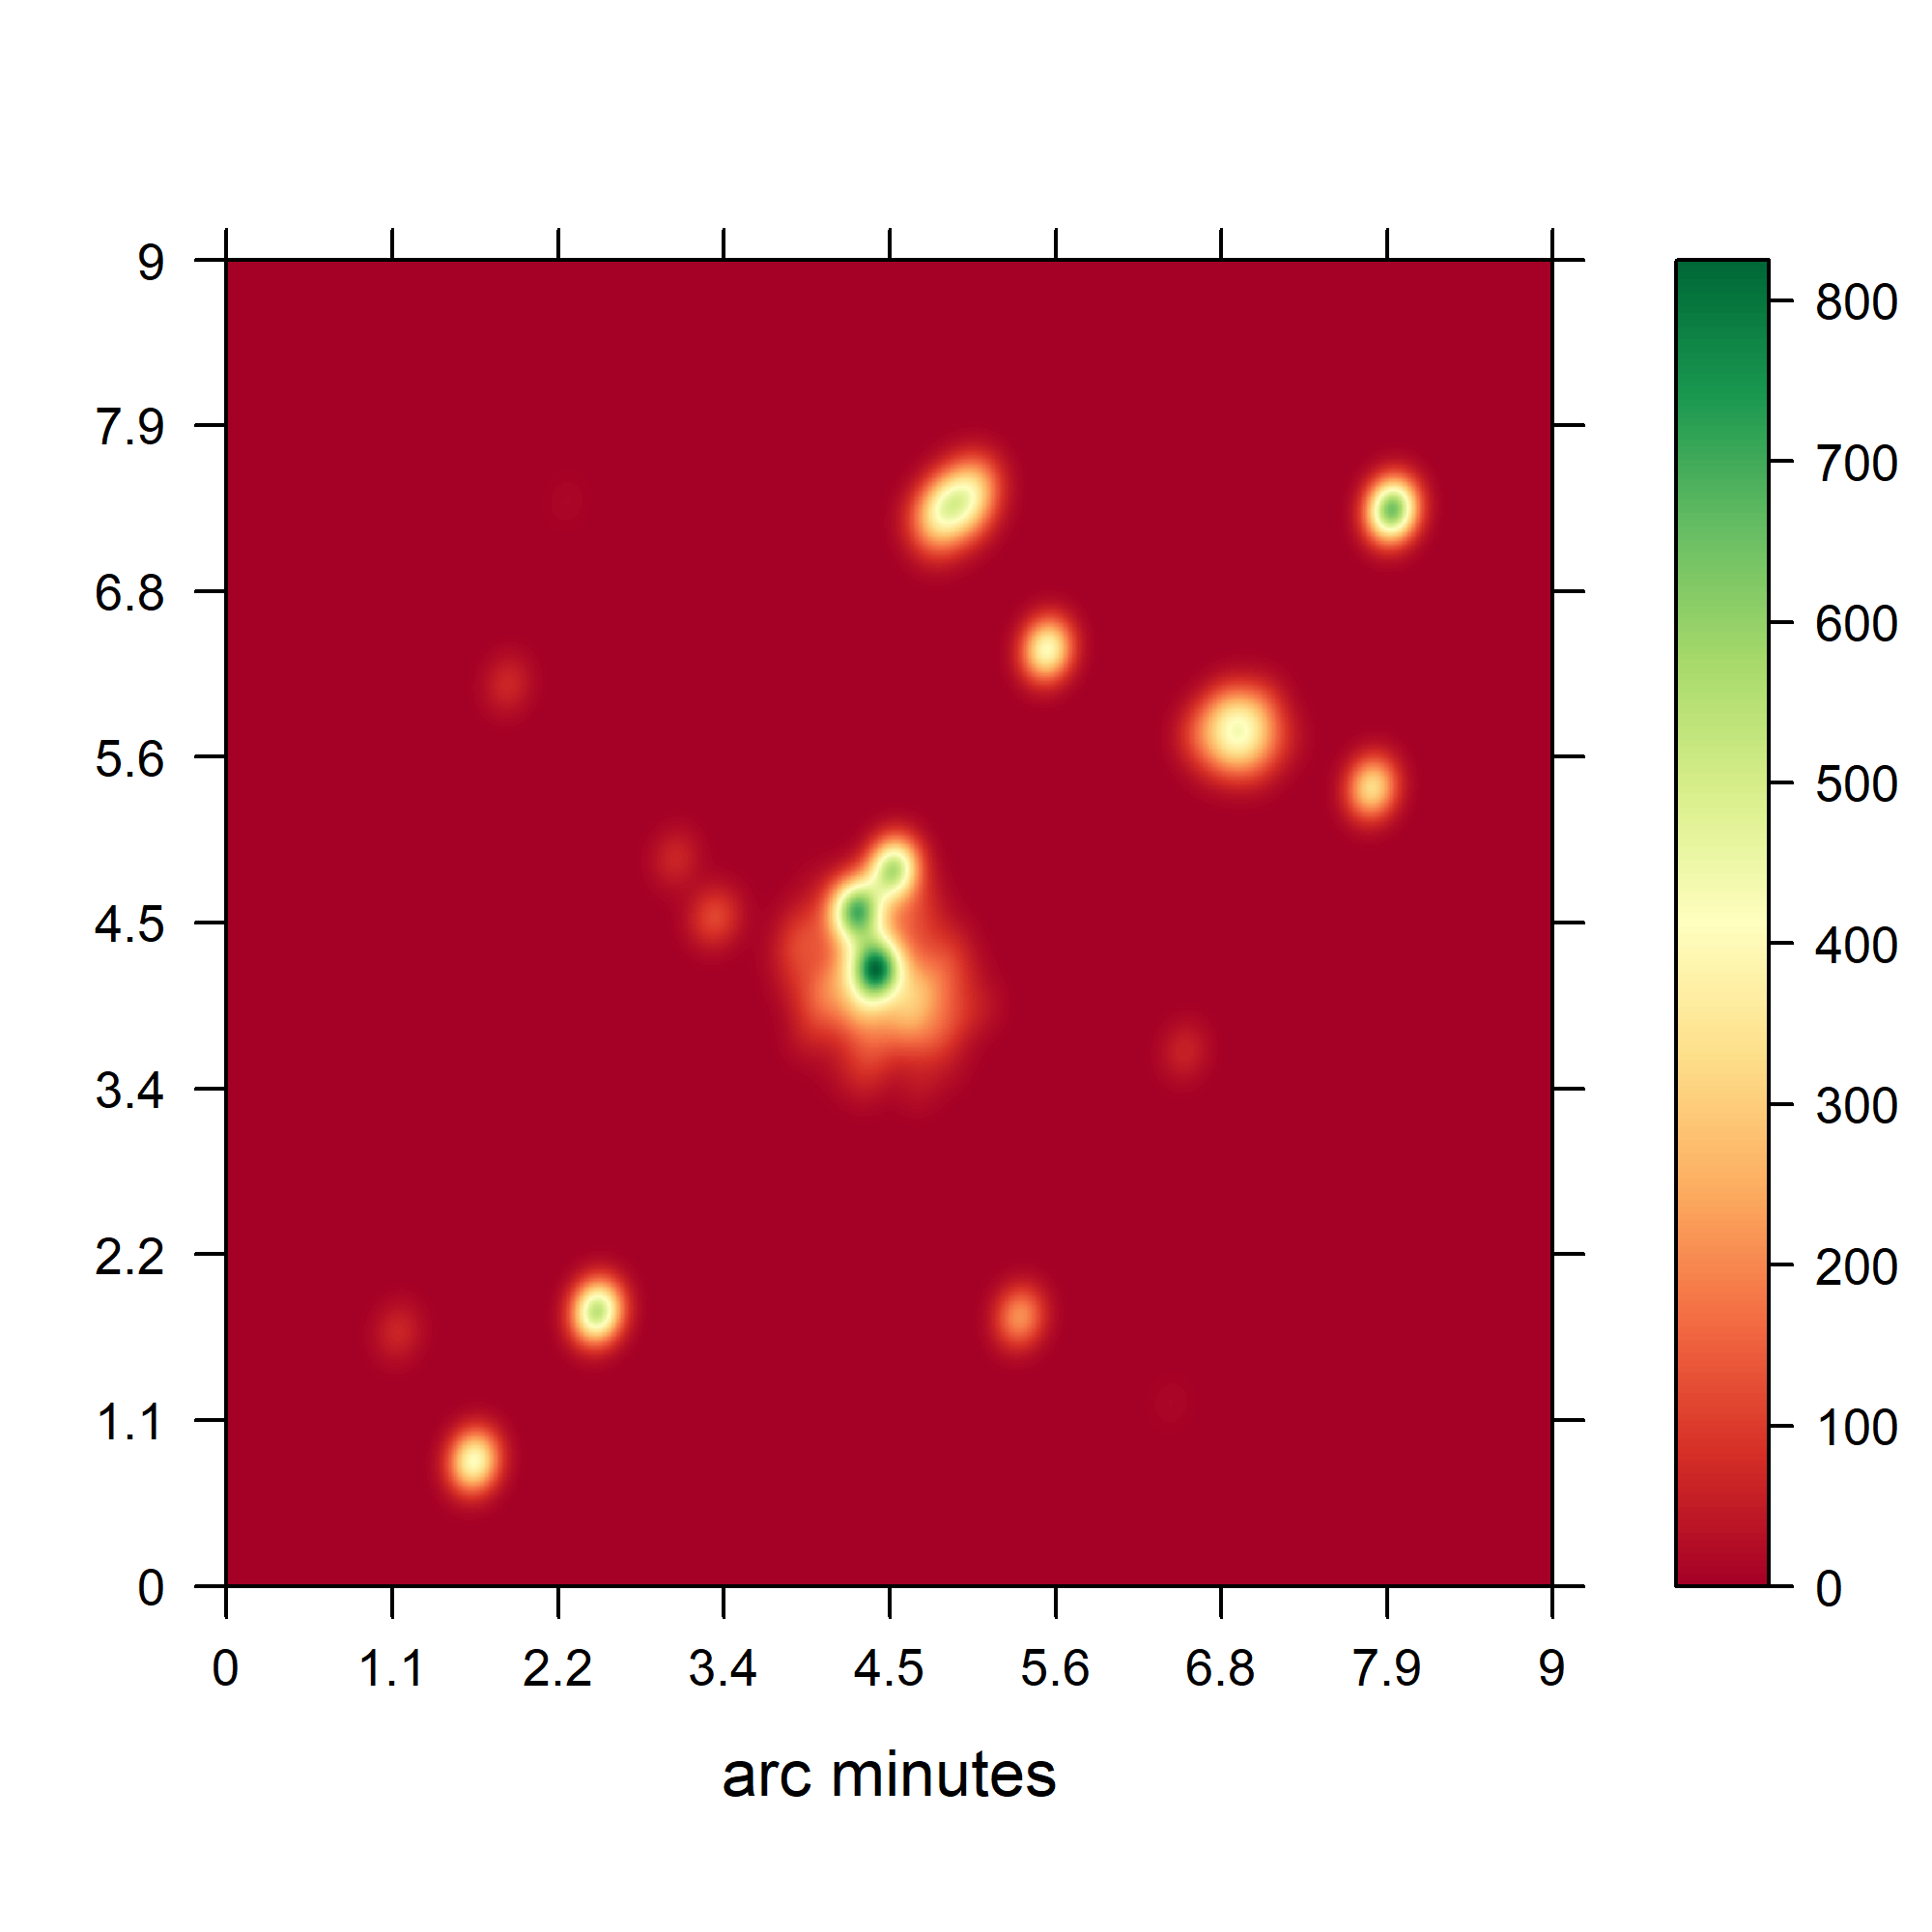
\includegraphics[width=\linewidth, trim={0.2in, 0.2in, 0, 0.2in}, clip]{./chapters/20.results/mixed/mixed_clean.png}
		\caption{CLEAN reconstruction}
		\label{results:mixed:tclean}
	\end{subfigure}
	\begin{subfigure}[b]{0.4\linewidth}
		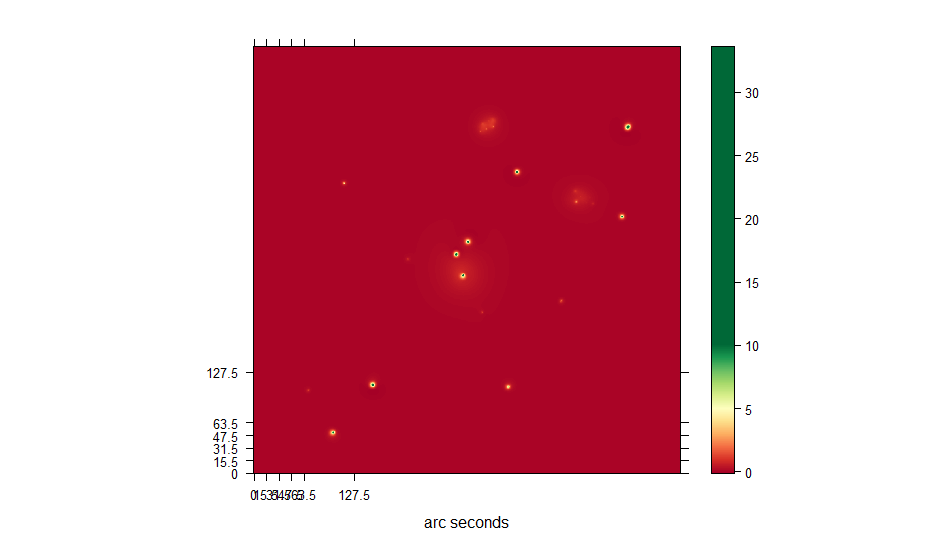
\includegraphics[width=\linewidth, trim={0.2in, 0.2in, 0, 0.2in}, clip]{./chapters/20.results/mixed/mixed_cd.png}
		\caption{Coordinate Descent Reconstruction}
		\label{results:mixed:cd}
	\end{subfigure}
	\caption{Reconstruction on mixed sources}
	\label{results:mixed}
\end{figure}

Question of Flux reconstruction

 $\lambda$ for different starlet layers like in \cite{girard2015sparse}

\begin{figure}[h]
	\centering
	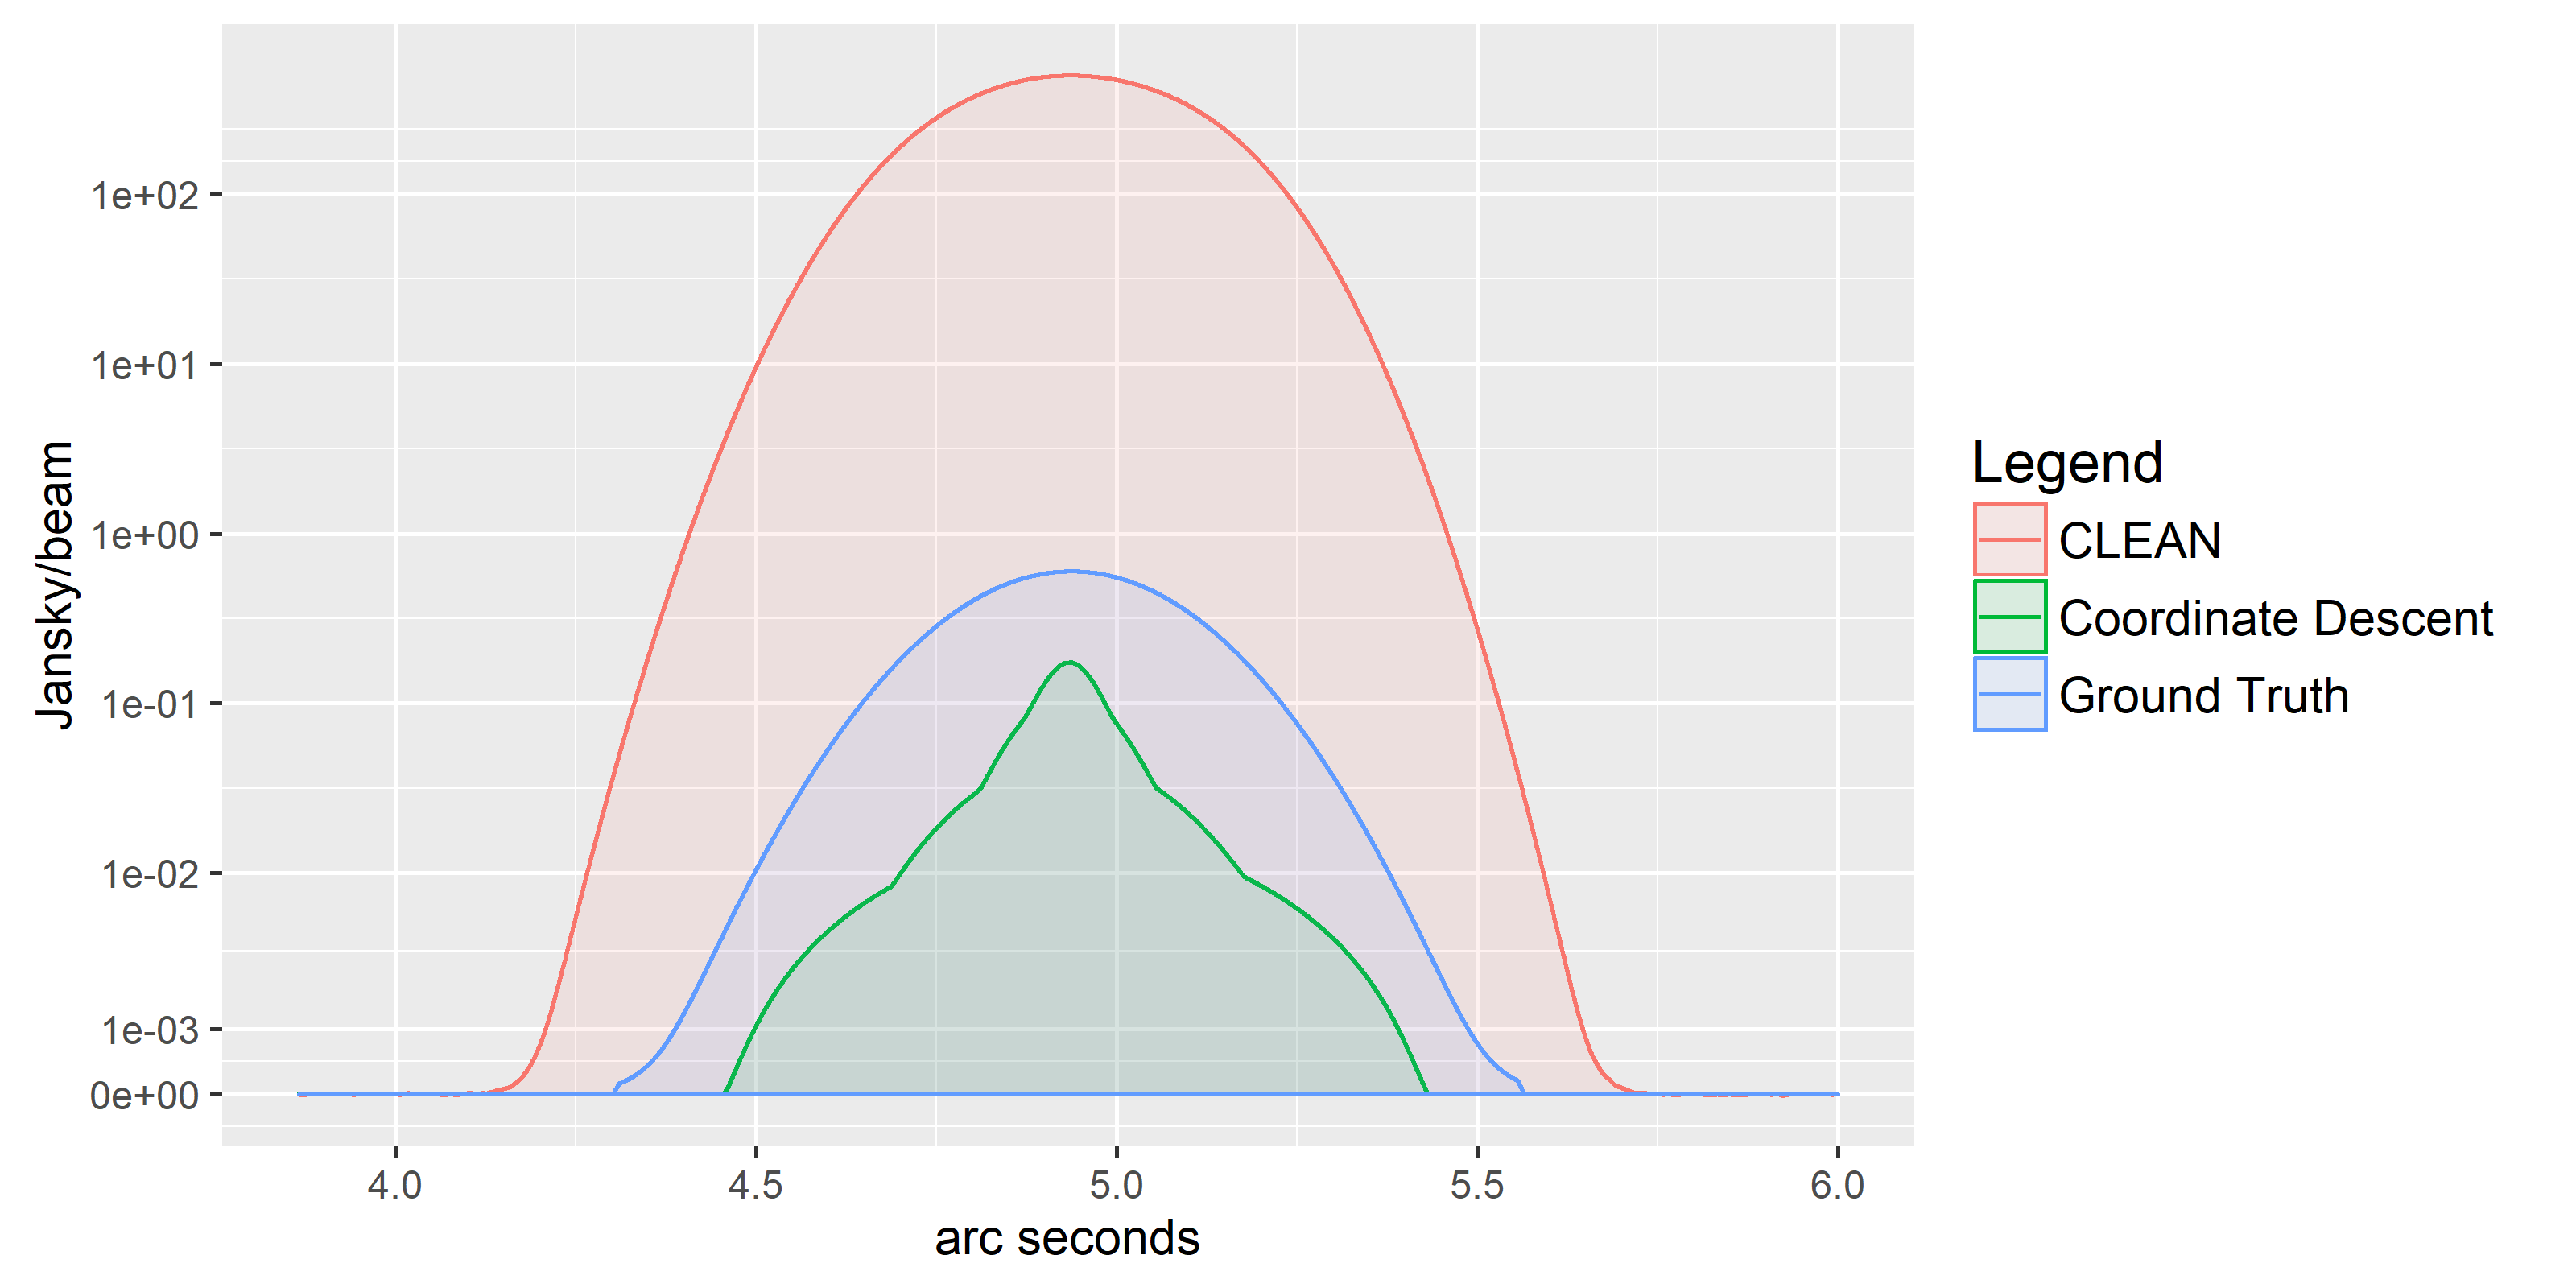
\includegraphics[width=0.8\linewidth]{./chapters/20.results/mixed/mixed_cut0.png}
	\caption{Reconstruction on mixed sources}
	\label{results:mixed:contour}
\end{figure}

Coordinate Descent did not reconstruct all point sources. How many starlets are non-zero is the major point for runtime. It depends on how many areas of the image are non-zero. Starlet has a representation for extended emission, how many starlets are needed for modelling is hard.

Runtime problems
1900 non-zero starlets, 



\newpage
\section{Compressed Sensing Reconstructions in the MeerKAT era}
Compressed Sensing and CLEAN based algorithms both use the non-uniform FFT to cycle between Visibility and image space. In this environment, Compressed Sensing needs more cycles to converge than CLEAN. This leads to iterative Compressed Sensing algorithms, which becomes difficult to distribute for the large scale MeerKAT problems. We postulated that one may reduce the runtime cost of Compressed Sensing reconstructions by replacing the non-uniform FFT approximation. Three alternatives were discussed: Optimal Projection on a uniform Grid, using Spherical Wave Harmonics and the direct Fourier Transform.

The optimal projection on a uniform grid is way of reducing the problem to a more manageable size. The grid size is usually a fraction of the original non-uniform measurements for MeerKAT reconstructions. The first step is to search for the optimal projection of Visibilities on a uniform grid. We then reconstruct the image with uniformly sampled Visibilities and do not need the original measurements. However, self-calibration requires a transformation from uniform sampled grid back to the original measurements. Unless one finds a way to project the calibration problem on a uniform grid too, self-calibration destroys the main advantage of this approach.

The second alternative is using Spherical Wave Harmonics instead of the Fourier Transform. It is a new way to represent the Radio Interferometric Measurement Equation and has only recently gained attention again. We analysed published research in this area\cite{carozzi2015imaging, mcewen2008simulating} and see potential for a new reconstruction architecture, which may reduce the overall runtime costs. At this point, it is unclear if or how many imaging problems have to be re-investigated by moving to Spherical Wave Harmonics. The Fourier Transform, self-calibration and the current formalism for Radio Interferometric Measurement equation is based on the plane wave\cite{smirnov2011revisiting}. Spherical Wave Harmonics are not. A real-world reconstruction algorithm with Spherical Wave Harmonics may have to deal with imaging problems in a fundamentally different way.

The last alternative, the direct Fourier Transform, uses the explicit matrix instead of an approximation algorithm. Previous attempts\cite{hardy2013direct} lead to an impractically large matrix for MeerKAT reconstructions, but showed potential for distributed computing. In this project, we improved the runtime costs and memory requirement of the direct Fourier Transform. We used Coordinate Descent together with the starlet transform and created an algorithm which only calculates the direct Fourier Transform for non-zero basis functions. Sadly, our improvements alone were not enough to scale the direct Fourier Transform to MeerKATs data volume. Compared to the non-uniform FFT based algorithms, our approach leads to higher runtime costs for the same measurements. 

In this project we have not found a clear alternative to the non-uniform FFT. It is readily available and currently seems to be the most efficient approximation of the Fourier Transform. The $w$-stacking algorithm\cite{offringa2014wsclean} has introduced some level of distribution for the non-uniform FFT operation, and state-of-the-art Compressed Sensing algorithms\cite{dabbech2018cygnus, pratley2018fast} are developed with distributed computing in mind. Still, the non-uniform FFT tends to dominate the runtime for large scale reconstructions. How to effectively distribute a reconstruction algorithm based on the non-uniform FFT is still an open problem.

With an expansion of the MeerKAT instrument already planned, the problem sizes will only increase in the near future. This may force reconstruction algorithms to increasingly rely on approximations instead of exact operations. Indeed, the path to a scalable, distributable reconstruction algorithm may lie in specialized approximations for MeerKAT. The large number of Visibilities is bound to contain redundant information. By increasing the data volume, it also potentially increases the amount of redundant information. The runtime costs of large scale reconstruction algorithms can be reduced by accounting for the inherent redundancy. The non-uniform FFT is a general purpose approximation\cite{kunisnonequispaced} and does not improve significantly by accounting for the redundancy.

Other alternatives, like the direct Fourier Transform, benefit from removing the redundant information. Depending on how much information is redundant, we might arrive at a more efficient Fourier Transform approximation. But as we have seen in this project, simply replacing the non-uniform FFT is not enough. Every alternative needs novel ways of introducing efficient approximations. The question whether the non-uniform FFT can be beat depends in certain cases on how redundant the information really is. 


This part is not really investigated in the Radio Astronomy Community. The non-uniform FFT is the staple, and alterantives are at least rarely published.

The Fourier approximation cannot be looked at without a reconstruction algorithm. In combinations, we may find an optimum which both is cheap and easy to distribute. This is the golden algorithm. The problem is that we only see potential for many different directions. At this point, there are many ways to potentially improve, but no overall goal.


Other ways of approximating the Fourier Transform have potential to improve Compressed Sensing reconstructions fundamentally. But as it is, there is no clear path to get to a better reconstruction algorithm. 








\newpage
\bibliography{mybib}{}
%\bibliographystyle{plain}
\bibliographystyle{unsrt}
\newpage
\listoffigures
\listoftables

\newpage
\input{./chapters/99.attachment/attachment.tex}
\newpage
\section{Ehrlichkeitserklärung}
Hiermit erkläre ich, dass ich die vorliegende schriftliche Arbeit
selbstständig und nur unter Zuhilfenahme der in den Verzeichnissen oder
in den Anmerkungen genannten Quellen angefertigt habe. Ich versichere
zudem, diese Arbeit nicht bereits anderweitig als Leistungsnachweis
verwendet zu haben. Eine Überprüfung der Arbeit auf Plagiate unter
Einsatz entsprechender Software darf vorgenommen werden.\\
Windisch, \today\\[4\baselineskip]
Jonas Schwammberger 

\end{document}